\documentclass[12pt,a4paper,oneside]{book}

% 1. Master Style for SCIRBRU Eastern Agri-Aqua AIoT (RBRU Masterclass Standard)
\usepackage{styles/scirbru_aiot_style}

% 2. Font configuration for XeLaTeX (Thai Unicode Sarabun)
\usepackage{fontspec}
\setmainfont{Sarabun}
\setsansfont{Sarabun}
\setmonofont{Sarabun}[Scale=0.9]

% 3. Hyperref Setup
\usepackage{hyperref}
\hypersetup{
    colorlinks=true,
    linkcolor=rbruNavy,
    citecolor=agriForest,
    urlcolor=aquaCyan,
    filecolor=durianGold,
    pdftitle={หลักสูตรเกษตรดิจิทัลและปัญญาประดิษฐ์ฝังตัว - มหาวิทยาลัยราชภัฏรำไพพรรณี},
    pdfauthor={ผู้ช่วยศาสตราจารย์ ดร.ชีวะ ทัศนา และคณะ}
}

\begin{document}

% ==========================================
% ส่วนนำ (Frontmatter)
% ==========================================
\frontmatter
% ============================================================
% ปกหน้าตำราวิชาการ (Academic Book Cover)
% มาตรฐาน มหาวิทยาลัยราชภัฏรำไพพรรณี
% ============================================================
\thispagestyle{empty}
\begin{titlepage}
\begin{tikzpicture}[remember picture, overlay]
    % พื้นหลังหลักไล่ระดับสีน้ำเงินราชภัฏ
    \fill[left color=rbruNavy!98!black, right color=rbruNavy!88!agriForest] 
        (current page.south west) rectangle (current page.north east);
    
    % แถบขลิบทองราชภัฏแนวตั้งทางซ้าย
    \fill[color=rbruGold] 
        ([xshift=2.4cm]current page.south west) rectangle ([xshift=2.6cm]current page.north west);

    % เส้นเรขาคณิตเวกเตอร์ฟิสิกส์คณิตศาสตร์โปร่งแสง
    \draw[color=white, opacity=0.08, line width=1.0pt]
        ([xshift=3.5cm, yshift=-2.5cm]current page.north west) -- ([xshift=-1.5cm, yshift=5cm]current page.south east);
    \draw[color=rbruGold, opacity=0.12, line width=1.2pt]
        ([xshift=3.5cm, yshift=-6cm]current page.north west) -- ([xshift=-1cm, yshift=2cm]current page.south east);

    % ข้อมูลสังกัดด้านบน
    \node[anchor=north west, text width=14.5cm] at ([xshift=3.2cm, yshift=-2.0cm]current page.north west) {
        {\fontsize{14}{18}\selectfont\bfseries\color{rbruGold} คณะวิทยาศาสตร์และเทคโนโลยี มหาวิทยาลัยราชภัฏรำไพพรรณี\par}
        \vspace{2pt}
        {\fontsize{10}{13}\selectfont\color{softMist!85} โครงการพัฒนาทักษะวิชาชีพชั้นสูงเพื่อการขับเคลื่อนเศรษฐกิจฐานนวัตกรรม (AIoT 2570)\par}
    };

    % ส่วนชื่อเรื่องหลัก (Main Title Block)
    \node[anchor=north west, text width=15.2cm] at ([xshift=3.2cm, yshift=-3.4cm]current page.north west) {
        {\color{rbruGold}\rule{0.45\textwidth}{3pt}\par}
        \vspace{8pt}
        {\fontsize{28}{35}\selectfont\bfseries\color{white} หลักสูตรเกษตรดิจิทัล\par}
        \vspace{3pt}
        {\fontsize{26}{33}\selectfont\bfseries\color{white} และปัญญาประดิษฐ์ฝังตัว\par}
        \vspace{7pt}
        {\fontsize{15}{21}\selectfont\bfseries\color{durianGold} สวนผลไม้มูลค่าสูงและการเพาะเลี้ยงสัตว์น้ำชายฝั่ง ภาคตะวันออก\par}
        \vspace{5pt}
        {\fontsize{9}{13}\selectfont\color{softMist!85} Digital Agriculture and Embedded Artificial Intelligence Curriculum\\for High-Value Fruit Orchards and Coastal Aquaculture\par}
        \vspace{8pt}
        {\color{rbruGold}\rule{0.75\textwidth}{1.2pt}\par}
    };

    % กรอบภาพศิลป์ปก Masterclass (Cover Artwork Window)
    \node[anchor=center, draw=rbruGold, line width=2.0pt, rounded corners=6pt, inner sep=0pt, fill=black] 
        at ([xshift=1.0cm, yshift=-1.0cm]current page.center) {
        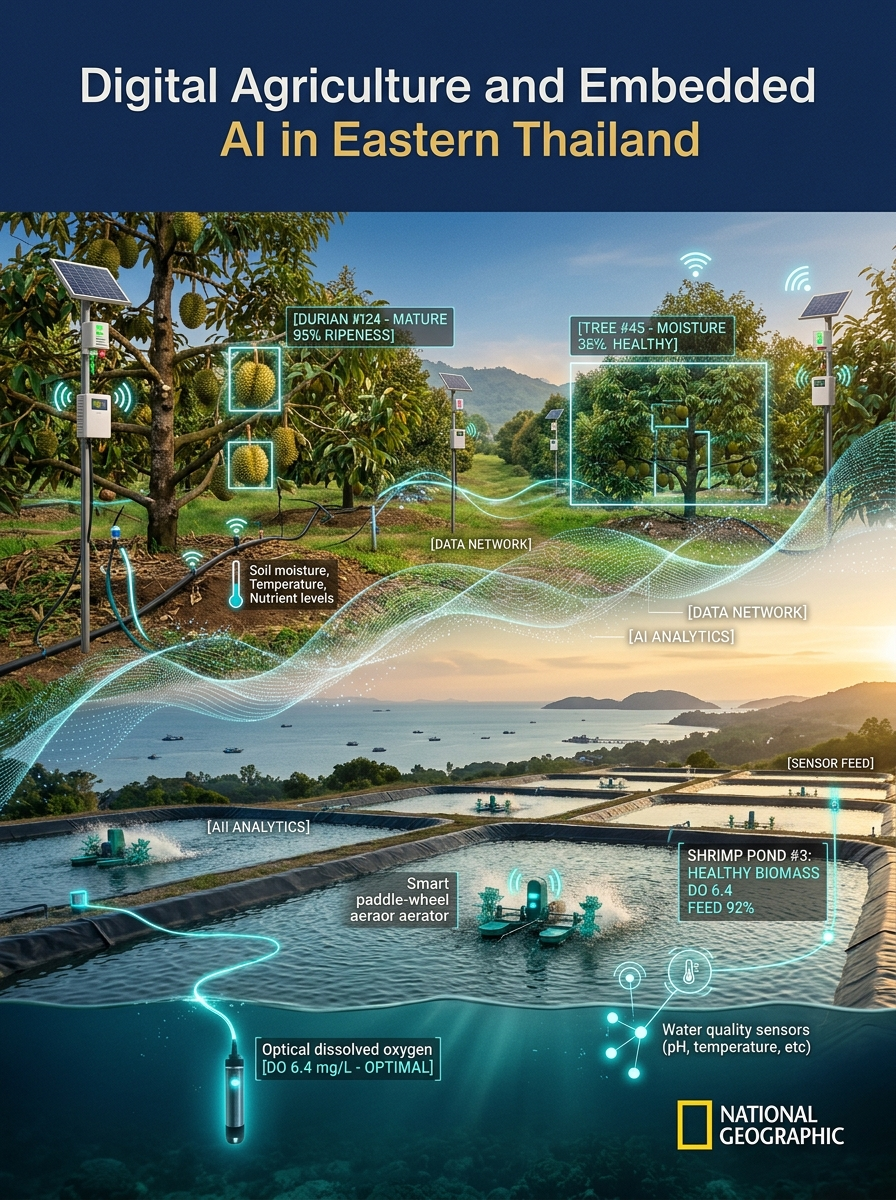
\includegraphics[width=14.5cm, height=9.2cm, keepaspectratio=false]{figures/cover_artwork.jpg}
    };

    % รายนามคณะผู้เขียนและสำนักพิมพ์ด้านล่าง
    \node[anchor=south west, text width=14.5cm] at ([xshift=3.2cm, yshift=1.8cm]current page.south west) {
        {\fontsize{12}{15}\selectfont\bfseries\color{white} ผู้ช่วยศาสตราจารย์ ดร.ชีวะ ทัศนา\par}
        \vspace{2pt}
        {\fontsize{9.5}{12}\selectfont\color{softMist!90} ร่วมกับคณะวิทยากรผู้ทรงคุณวุฒิ คณะวิทยาศาสตร์และเทคโนโลยี\par}
        \vspace{2pt}
        {\fontsize{8.5}{11}\selectfont\color{softMist!75} ผศ.อรรถกร คำฉัตร \textbar\ ผศ.ดร.ณมนรัก คำฉัตร \textbar\ รศ.ดร.นิภัทร เปี่ยมอรุณ \textbar\ ผศ.ดร.จิรภัทร จันทมาลี\par}
        {\fontsize{8.5}{11}\selectfont\color{softMist!75} ผศ.นิคม รัตนโรจนกุล \textbar\ รศ.ดร.นันทพร มูลรังษี \textbar\ ผศ.ดร.สุพัตรา รักษาพรต\par}
        \vspace{10pt}
        {\color{rbruGold}\rule{0.35\textwidth}{0.8pt}\par}
        \vspace{4pt}
        {\fontsize{10}{13}\selectfont\bfseries\color{rbruGold} สำนักพิมพ์มหาวิทยาลัยราชภัฏรำไพพรรณี \quad \textbar \quad \color{softMist!80}พ.ศ. 2570\par}
    };
\end{tikzpicture}
\end{titlepage}
\clearpage

% ============================================================
% หน้ารองปก (Title Page)
% ============================================================
\thispagestyle{empty}
\begin{center}
    \vspace*{1.5cm}
    
    {\color{rbruNavy}\rule{0.65\textwidth}{2pt}}
    \vspace{0.8cm}
    
    {\fontsize{24}{30}\selectfont\bfseries\color{rbruNavy} หลักสูตรเกษตรดิจิทัลและปัญญาประดิษฐ์ฝังตัว\par}
    \vspace{0.3cm}
    {\fontsize{18}{24}\selectfont\bfseries\color{durianGold} สวนผลไม้มูลค่าสูงและการเพาะเลี้ยงสัตว์น้ำชายฝั่ง ภาคตะวันออก\par}
    \vspace{0.5cm}
    {\fontsize{12}{16}\selectfont\color{slateGrey} Digital Agriculture and Embedded Artificial Intelligence Curriculum for High-Value Fruit Orchards and Coastal Aquaculture\par}
    
    \vspace{0.8cm}
    {\color{rbruGold}\rule{0.45\textwidth}{1.5pt}}
    
    \vspace{2.0cm}
    
    {\fontsize{15}{20}\selectfont\bfseries\color{rbruNavy} ผู้ช่วยศาสตราจารย์ ดร.ชีวะ ทัศนา\par}
    {\fontsize{12}{16}\selectfont ปร.ด. (ฟิสิกส์ประยุกต์) สถาบันเทคโนโลยีพระจอมเกล้าเจ้าคุณทหารลาดกระบัง\par}
    {\fontsize{12}{16}\selectfont อาจารย์ประจำสาขาวิชาฟิสิกส์และวิทยาศาสตร์ทั่วไป คณะวิทยาศาสตร์และเทคโนโลยี\par}
    
    \vspace{1.0cm}
    
    {\fontsize{13}{18}\selectfont\bfseries\color{agriForest} ร่วมกับคณะวิทยากรผู้เชี่ยวชาญ คณะวิทยาศาสตร์และเทคโนโลยี\par}
    \vspace{0.3cm}
    \begin{tabular}{ll}
        \textbf{ผู้ช่วยศาสตราจารย์ อรรถกร คำฉัตร} & วท.ม. (เทคโนโลยีสารสนเทศ) \\
        \textbf{ผู้ช่วยศาสตราจารย์ ดร.ณมนรัก คำฉัตร} & ปร.ด. (ชีววิทยา/พืชศาสตร์) \\
        \textbf{รองศาสตราจารย์ ดร.นิภัทร เปี่ยมอรุณ} & ปร.ด. (เคมีประยุกต์ / เคมีเชิงฟิสิกส์) \\
        \textbf{ผู้ช่วยศาสตราจารย์ ดร.จิรภัทร จันทมาลี} & ปร.ด. (จุลชีววิทยา) \\
        \textbf{ผู้ช่วยศาสตราจารย์ นิคม รัตนโรจนกุล} & วท.ม. (ฟิสิกส์ประยุกต์) \\
        \textbf{รองศาสตราจารย์ ดร.นันทพร มูลรังษี} & ปร.ด. (เคมีวิเคราะห์) \\
        \textbf{ผู้ช่วยศาสตราจารย์ ดร.สุพัตรา รักษาพรต} & ปร.ด. (เทคโนโลยีเคมี) \\
    \end{tabular}
    
    \vfill
    
    {\color{rbruNavy}\rule{0.35\textwidth}{1pt}}
    \vspace{0.4cm}
    {\fontsize{13}{16}\selectfont\bfseries\color{rbruNavy} คณะวิทยาศาสตร์และเทคโนโลยี มหาวิทยาลัยราชภัฏรำไพพรรณี\par}
    {\fontsize{11}{14}\selectfont พ.ศ. 2570\par}
    \vspace{1.0cm}
\end{center}
\clearpage

\chapter*{คำนำ}
\addcontentsline{toc}{chapter}{คำนำ}

ตำราวิชาการเรื่อง \textbf{หลักสูตรเกษตรดิจิทัลและปัญญาประดิษฐ์ฝังตัว สวนผลไม้มูลค่าสูงและการเพาะเลี้ยงสัตว์น้ำชายฝั่ง ภาคตะวันออก} เล่มนี้ เรียบเรียงขึ้นเพื่อใช้เป็นตำราและเอกสารประกอบการฝึกอบรมขั้นสูงในโครงการพัฒนาบัณฑิตพันธุ์ใหม่และกำลังคนสมรรถนะสูงเพื่อตอบโจทย์ภาคการผลิตตามนโยบายการปฏิรูปการอุดมศึกษาไทย โดยมุ่งเน้นการบูรณาการองค์ความรู้ทางฟิสิกส์ประยุกต์ เคมีเชิงฟิสิกส์ วิทยาการคอมพิวเตอร์ และเทคโนโลยีปัญญาประดิษฐ์ฝังตัว (Embedded AI และ Edge Computing) เข้ากับบริบทการแก้ปัญหาจริงในแปลงเกษตรกรรมและฟาร์มเพาะเลี้ยงสัตว์น้ำเศรษฐกิจของภาคตะวันออก

พื้นที่ภาคตะวันออกของประเทศไทย โดยเฉพาะจังหวัดจันทบุรี ระยอง และตราด ถือเป็นศูนย์กลางทางเศรษฐกิจการเกษตรที่สำคัญอย่างยิ่ง ทั้งในด้านการผลิตผลไม้เมืองร้อนมูลค่าสูง เช่น ทุเรียน มังคุด และเงาะ รวมทั้งเป็นแหล่งเพาะเลี้ยงสัตว์น้ำชายฝั่งที่สำคัญ เช่น กุ้งขาวแวนนาไมและปลากะพงขาว อย่างไรก็ดี เกษตรกรและผู้ประกอบการต้องเผชิญกับความท้าทายเชิงโครงสร้าง ทั้งปัญหาการเปลี่ยนแปลงสภาพภูมิอากาศ ความผันผวนของต้นทุนพลังงานไฟฟ้า แรงงานขาดแคลน และข้อกำหนดด้านมาตรฐานคุณภาพผลผลิตส่งออกที่เข้มงวด การทำการเกษตรแบบพึ่งพาประสบการณ์ดั้งเดิมเพียงอย่างเดียวจึงไม่เพียงพอต่อการรักษาขีดความสามารถในการแข่งขัน

คณะผู้เขียนจึงได้สังเคราะห์กรอบการทำงานเชิงระบบโดยแบ่งออกเป็นสองกิจกรรมหลัก ได้แก่
\begin{enumerate}
    \item \textbf{กิจกรรมที่ 1 นวัตกร AIoT สวนผลไม้มูลค่าสูง} มุ่งเน้นการตรวจวัดความสมบูรณ์ของดินและสภาพอากาศด้วยโพรบ 7-in-1 การประเมินค่าแรงดึงระเหยน้ำของอากาศ (VPD) การคำนวณการใช้น้ำของพืช ($ET_c$) ตามระยะฟีโนโลยี การควบคุมระบบไฮดรอลิกส์ด้วยวาล์วไฟฟ้า 24VAC ป้องกันปรากฏการณ์ Water Hammer การประเมินความสุกแก่ของทุเรียนด้วยคอมพิวเตอร์วิทัศน์สีหนามร่องพูและการสั่นพ้องของคลื่นเสียง และระบบคัดเกรดผลไม้อัตโนมัติบนสายพานด้วยโมเดล YOLO
    \item \textbf{กิจกรรมที่ 2 นวัตกร AIoT ฟาร์มเพาะเลี้ยงสัตว์น้ำชายฝั่ง} มุ่งเน้นการตรวจวัดคุณภาพน้ำแบบเรียลไทม์ด้วยโพรบวัดออกซิเจนละลายเชิงแสง (Optical DO) และความเค็ม การคำนวณอุณหพลศาสตร์การละลายของออกซิเจน (Benson-Krause Model) การควบคุมมอเตอร์เครื่องตีน้ำด้วยอินเวอร์เตอร์ VFD ผ่านโปรโตคอล Modbus RTU เพื่อประหยัดพลังงานไฟฟ้าได้ถึงร้อยละ 40 การวิเคราะห์ปริมาณอาหารเหลือก้นบ่อบนยอยกอาหารกุ้งด้วยคอมพิวเตอร์วิทัศน์ และระบบเตือนภัยฉุกเฉินตลอด 24 ชั่วโมง
\end{enumerate}

คณะผู้เขียนหวังเป็นอย่างยิ่งว่า ตำราเล่มนี้จะเป็นประโยชน์ต่อนักศึกษา นักวิจัย คณาจารย์ เกษตรกรปราดเปรื่อง (Smart Farmers) และผู้สนใจทั่วไป ในการนำองค์ความรู้ไปประยุกต์สร้างสรรค์นวัตกรรมเพื่อยกระดับการเกษตรแม่นยำและการเพาะเลี้ยงสัตว์น้ำของประเทศอย่างยั่งยืนสืบไป

\vspace{1.5cm}
\begin{flushright}
    \textbf{ผู้ช่วยศาสตราจารย์ ดร.ชีวะ ทัศนา}\\
    คณะวิทยาศาสตร์และเทคโนโลยี มหาวิทยาลัยราชภัฏรำไพพรรณี\\
    กันยายน 2570
\end{flushright}
\clearpage

\chapter*{กิตติกรรมประกาศ}
\addcontentsline{toc}{chapter}{กิตติกรรมประกาศ}

การจัดทำตำราวิชาการและชุดเอกสารหลักสูตรเล่มนี้ สำเร็จลุล่วงได้อย่างสมบูรณ์ด้วยความร่วมมือ ร่วมแรง และร่วมใจจากคณาจารย์ นักวิจัย และบุคลากรของคณะวิทยาศาสตร์และเทคโนโลยี มหาวิทยาลัยราชภัฏรำไพพรรณี ที่ได้ร่วมกันถ่ายทอดองค์ความรู้และประสบการณ์วิจัยเชิงประยุกต์ตลอดระยะเวลากว่าทศวรรษ

คณะผู้เขียนขอกราบขอบพระคุณคณะผู้บริหารมหาวิทยาลัยราชภัฏรำไพพรรณี และคณบดีคณะวิทยาศาสตร์และเทคโนโลยี ที่ได้ให้การสนับสนุนด้านนโยบาย งบประมาณ และสิ่งอำนวยความสะดวกในการวิจัยพัฒนา รวมถึงห้องปฏิบัติการวิทยาศาสตร์และฟาร์มทดสอบต้นแบบ

ขอขอบพระคุณคณะวิทยากรผู้ทรงคุณวุฒิทุกท่าน ได้แก่ ผู้ช่วยศาสตราจารย์ อรรถกร คำฉัตร, ผู้ช่วยศาสตราจารย์ ดร.ณมนรัก คำฉัตร, รองศาสตราจารย์ ดร.นิภัทร เปี่ยมอรุณ, ผู้ช่วยศาสตราจารย์ ดร.จิรภัทร จันทมาลี, ผู้ช่วยศาสตราจารย์ นิคม รัตนโรจนกุล, รองศาสตราจารย์ ดร.นันทพร มูลรังษี และผู้ช่วยศาสตราจารย์ ดร.สุพัตรา รักษาพรต ที่ได้สละเวลาทุ่มเทจัดเตรียมเนื้อหาวิชาการ ตรวจสอบความถูกต้องทางวิทยาศาสตร์ และพัฒนาระบบซอฟต์แวร์ต้นแบบภาคสนาม

ขอขอบพระคุณเครือข่ายแปลงวิจัยและชาวสวนผลไม้ในจังหวัดจันทบุรี ตราด และระยอง รวมถึงผู้ประกอบการฟาร์มเพาะเลี้ยงกุ้งขาวและสัตว์น้ำชายฝั่ง ที่ได้เอื้อเฟื้อพื้นที่ในการเก็บตัวอย่างดิน สภาพแวดล้อมทางชลศาสตร์ และการทดสอบระบบสมองกลฝังตัวหน้างานจริง ซึ่งทำให้ข้อมูลและผลการทดลองในตำราเล่มนี้มีความน่าเชื่อถือและสอดคล้องกับสภาพปัญหาที่แท้จริง

คุณงามความดีและประโยชน์อันพึงมีจากตำราเล่มนี้ คณะผู้เขียนขอน้อมอุทิศแด่บูรพาจารย์ ผู้มีพระคุณ และสถาบันการศึกษาทุกแห่งที่ได้ประสิทธิ์ประสาทวิชาความรู้ให้แก่คณะผู้เขียนเสมอมา

\vspace{1.5cm}
\begin{flushright}
    \textbf{คณะผู้จัดทำหลักสูตร AIoT 2570}\\
    มหาวิทยาลัยราชภัฏรำไพพรรณี
\end{flushright}
\clearpage

\chapter*{แผนบริหารการสอนประจำวิชา}
\addcontentsline{toc}{chapter}{แผนบริหารการสอนประจำวิชา}

\noindent\textbf{รหัสและชื่อวิชา}\\
หลักสูตรเกษตรดิจิทัลและปัญญาประดิษฐ์ฝังตัวสำหรับการจัดการสวนผลไม้มูลค่าสูงและการเพาะเลี้ยงสัตว์น้ำชายฝั่ง ภาคตะวันออก (Eastern Digital Agriculture and Embedded Artificial Intelligence: AIoT for High-Value Fruit Orchards and Coastal Aquaculture)

\vspace{0.3cm}
\noindent\textbf{จำนวนหน่วยกิตและชั่วโมงการเรียนรู้}\\
จำนวนรวม 120 ชั่วโมงการเรียนรู้ (บรรยายเชิงทฤษฎี 45 ชั่วโมง และปฏิบัติการภาคสนาม 75 ชั่วโมง)

\vspace{0.3cm}
\noindent\textbf{คำอธิบายรายวิชา}\\
การศึกษาและฝึกทักษะเชิงลึกเกี่ยวกับหลักการทางฟิสิกส์เกษตรและเคมีวิเคราะห์ เซนเซอร์วัดคุณภาพดิน สภาพอากาศ และคุณภาพน้ำชายฝั่ง สถาปัตยกรรมระบบสมองกลฝังตัวและการประมวลผลที่ขอบ (Edge Computing) ด้วยไมโครคอนโทรลเลอร์ประสิทธิภาพสูง การควบคุมวาล์วไฟฟ้าชลศาสตร์และการขับเคลื่อนมอเตอร์กำลังสูงด้วยอินเวอร์เตอร์ปรับความถี่ (VFD) การจำลองและออกแบบระบบชลศาสตร์ตามระยะฟีโนโลยีของพืชและการถ่ายเทมวลสารของก๊าซในน้ำ การเขียนโปรแกรมคอมพิวเตอร์วิทัศน์และการประมวลผลสัญญาณเสียงสำหรับการจำแนกความสุกแก่และการตรวจวินิจฉัยโรคพืชและสัตว์น้ำ โครงข่ายไร้สายระยะไกลพลังงานต่ำ (LoRaWAN) ร่วมกับพลังงานแสงอาทิตย์ และการบูรณาการพัฒนานวัตกรรมโครงงานภาคสนาม

\vspace{0.3cm}
\noindent\textbf{วัตถุประสงค์ทั่วไปของรายวิชา}\\
เมื่อผู้เรียนสำเร็จการศึกษาในรายวิชานี้แล้ว จะมีความรู้ความสามารถดังต่อไปนี้
\begin{enumerate}
    \item อธิบายหลักการทางฟิสิกส์และเคมีเชิงฟิสิกส์ที่เกี่ยวข้องกับการเจริญเติบโตของพืชสวนและสัตว์น้ำชายฝั่งได้อย่างถูกต้อง
    \item ออกแบบและต่อวงจรอุปกรณ์สมองกลฝังตัวร่วมกับเซนเซอร์อุตสาหกรรมและตัวขับกำลังสูงได้อย่างปลอดภัยตามมาตรฐานวิศวกรรม
    \item พัฒนาอัลกอริทึมปัญญาประดิษฐ์แบบ Two-Stage Decoupling สำหรับการประมวลผลภาพถ่ายและสัญญาณเสียงบนอุปกรณ์เอดจ์ได้อย่างมีประสิทธิภาพ
    \item ออกแบบและติดตั้งโครงข่ายสื่อสารไร้สาย IoT ที่ใช้พลังงานแสงอาทิตย์สำหรับพื้นที่ห่างไกลได้อย่างเหมาะสม
    \item บูรณาการองค์ความรู้สร้างสรรค์โครงงานนวัตกรรมแก้ปัญหาจริงในฟาร์มเกษตรกรรมและฟาร์มสัตว์น้ำได้อย่างสมบูรณ์
\end{enumerate}

\newpage

\noindent\textbf{แผนการจัดการเรียนรู้ 15 สัปดาห์}

\begin{table}[H]
\small
\centering
\caption*{ตารางแสดงแผนการจัดการเรียนรู้รายสัปดาห์}
\begin{tabularx}{\textwidth}{cp{3.2cm}p{5.5cm}Y}
    \toprule
    \textbf{สัปดาห์} & \textbf{หัวข้อการเรียนรู้} & \textbf{กิจกรรมและเนื้อหาเชิงปฏิบัติการ} & \textbf{วิทยากรผู้สอน} \\
    \midrule
    1 & ฟิสิกส์เกษตรและคุณภาพดิน & การอ่านค่า NPK/pH/EC ดิน 7-in-1 และการวิเคราะห์ค่า VPD & ผศ.ดร.ชีวะ ทัศนา \\
    2 & เซนเซอร์คุณภาพน้ำชายฝั่ง & การสอบเทียบหัววัด Optical DO และการชดเชยค่าความเค็ม & ผศ.ดร.สุพัตรา รักษาพรต \\
    3 & สมองกลฝังตัวและการควบคุม & การเขียนโปรแกรม ESP32-S3 คุมวาล์ว 24VAC และ FreeRTOS & ผศ.อรรถกร คำฉัตร \\
    4 & การขับเคลื่อนมอเตอร์กำลังสูง & การควบคุมอินเวอร์เตอร์ VFD ขับมอเตอร์ 3 เฟสผ่าน Modbus & ผศ.ดร.ชีวะ ทัศนา \\
    5 & ไฮดรอลิกส์ท่อและการให้น้ำ & การคำนวณ $ET_c$ ฟีโนโลยี และการสูญเสียแรงดันในท่อ & ผศ.ดร.ชีวะ ทัศนา \\
    6 & อุณหพลศาสตร์ออกซิเจนในน้ำ & สมการ Benson-Krause และการคำนวณอัตรา SOTR/OTR & รศ.ดร.นิภัทร เปี่ยมอรุณ \\
    7 & โครงข่ายไร้สายระยะสั้น & การเชื่อมต่อ ESP-NOW สองบอร์ด และเกตเวย์ MQTT LINE & ผศ.อรรถกร คำฉัตร \\
    8 & สถาปัตยกรรมคลาวด์เทเลเมทรี & การจัดเก็บข้อมูลบน TimescaleDB และแดชบอร์ดฟาร์มกุ้ง & ผศ.ดร.ชีวะ ทัศนา \\
    9 & คอมพิวเตอร์วิทัศน์ทุเรียน & การตัดแยกสีหนามร่องพูด้วยระบบ HSV และ Contour & รศ.ดร.นิภัทร เปี่ยมอรุณ \\
    10 & สวนศาสตร์เคาะเสียงทุเรียน & การประมวลผลสัญญาณเสียงด้วย FFT จำแนก \% เนื้อแห้ง & ผศ.ดร.ชีวะ ทัศนา \\
    11 & คอมพิวเตอร์วิทัศน์ยออาหาร & การประเมินพื้นที่เม็ดอาหารเหลือเพื่อปรับรอบออโต้ฟีดเดอร์ & ผศ.อรรถกร คำฉัตร \\
    12 & โมเดล YOLO คัดเกรดผลไม้ & การติดป้ายข้อมูลบน Roboflow และฝึกสอนโมเดล YOLO & ผศ.ดร.ชีวะ ทัศนา \\
    13 & AI วินิจฉัยโรคสัตว์น้ำและพืช & การจำแนกโรคกุ้ง WSSV และรากเน่าโคนเน่าทุเรียน & ผศ.ดร.จิรภัทร จันทมาลี \\
    14 & โครงข่าย LoRaWAN พลังงานแสง & การบีบอัดไบนารีและคำนวณขนาดแผงโซลาร์เซลล์ LiFePO4 & ผศ.ดร.ชีวะ ทัศนา \\
    15 & นำเสนอโครงงานบูรณาการ & การทดสอบระบบต้นแบบจริงภาคสนามและการประเมินผล & คณาจารย์ทุกท่าน \\
    \bottomrule
\end{tabularx}
\end{table}

\vspace{0.3cm}
\noindent\textbf{เกณฑ์การวัดและประเมินผลการเรียนรู้}\\
การประเมินผลการเรียนรู้แบ่งออกเป็น 3 ส่วน ได้แก่
\begin{enumerate}
    \item การทดสอบย่อยและใบงานปฏิบัติการประจำโมดูล ร้อยละ 30
    \item การเข้าร่วมกิจกรรมและทักษะการปฏิบัติงานภาคสนาม ร้อยละ 20
    \item โครงงานบูรณาการนวัตกรรมนวัตกร AIoT (Capstone Project) ร้อยละ 50
\end{enumerate}
\clearpage


% สารบัญหลัก สารบัญภาพ และสารบัญตาราง
\clearpage
\phantomsection
\addcontentsline{toc}{chapter}{\contentsname}
\tableofcontents

\clearpage
\phantomsection
\addcontentsline{toc}{chapter}{\listfigurename}
\listoffigures

\clearpage
\phantomsection
\addcontentsline{toc}{chapter}{\listtablename}
\listoftables

% ==========================================
% ส่วนเนื้อหา (Mainmatter)
% ==========================================
\mainmatter

% ตอนที่ 1: รากฐานฟิสิกส์เกษตรและสมองกลฝังตัว
\chapter{วิศวกรรมฟิสิกส์เกษตรดิจิทัล\index{ฟิสิกส์เกษตรดิจิทัล (Digital Agriphysics)}\index{Digital Agriphysics}และสรีรวิทยาพืชและสัตว์น้ำชายฝั่ง}
\label{chap:ch01}

\section*{แผนบริหารการสอนประจำบทที่ 1}
\addcontentsline{toc}{section}{แผนบริหารการสอนประจำบทที่ 1}

\begin{planbox}{หัวข้อเนื้อหาประจำบท}
\begin{enumerate}[topsep=2pt, itemsep=1pt, partopsep=0pt, parsep=0pt, leftmargin=1.5em]
    \item ความสำคัญของวิศวกรรมฟิสิกส์เกษตรดิจิทัลต่อการผลิตผลไม้มูลค่าสูงและการเพาะเลี้ยงสัตว์น้ำ
    \item รากฐานฟิสิกส์และเคมีไฟฟ้าของหัววัดสารอาหารและสภาพดินแบบบูรณาการ 7-in-1
    \item การแพร่ของก๊าซและอุณหพลศาสตร์แรงดึงระเหยน้ำของบรรยากาศสำหรับพืชสวน
    \item ฟิสิกส์การวัดออกซิเจนละลายน้ำเชิงแสงและสมดุลเคมีของน้ำในบ่อเพาะเลี้ยงสัตว์น้ำ
    \item โปรโตคอลการสื่อสารข้อมูลเซนเซอร์อุตสาหกรรมด้วย Modbus RTU\index{โปรโตคอลมอดบัส (Modbus RTU)}\index{Modbus RTU} ผ่านสายสัญญาณ RS485
\end{enumerate}
\end{planbox}

\begin{planbox}{วัตถุประสงค์เชิงพฤติกรรม}
\begin{enumerate}[topsep=2pt, itemsep=1pt, partopsep=0pt, parsep=0pt, leftmargin=1.5em]
    \item อธิบายสมการเนิร์นสต์และความสัมพันธ์เชิงฟิสิกส์ของหัววัดค่ากรด-ด่างและความเค็มได้อย่างถูกต้อง
    \item คำนวณค่าแรงดึงระเหยน้ำของอากาศจากอุณหภูมิและความชื้นสัมพัทธ์ได้อย่างแม่นยำ
    \item อธิบายหลักการดับการเรืองแสงเชิงแสงในการวัดออกซิเจนละลายน้ำได้อย่างถูกต้อง
    \item ออกแบบการเชื่อมต่อโครงข่ายเซนเซอร์ RS485 ร่วมกับการคำนวณรหัสตรวจสอบความถูกต้อง CRC-16 ได้อย่างสมบูรณ์
\end{enumerate}
\end{planbox}

\newpage

\begin{planbox}{วิธีสอนและกิจกรรมการเรียนการสอน}
\begin{enumerate}[topsep=2pt, itemsep=1pt, partopsep=0pt, parsep=0pt, leftmargin=1.5em]
    \item บรรยายหลักการทางฟิสิกส์ สรีรวิทยาพืช และสมดุลเคมีสิ่งแวดล้อมประกอบสื่อทัศนูปกรณ์
    \item สาธิตการสอบเทียบหัววัดดิน 7-in-1 และหัววัด Optical DO ด้วยสารละลายบัฟเฟอร์มาตรฐาน
    \item ปฏิบัติการทดลองวัดค่าจริงในตัวอย่างดินสวนทุเรียนและตัวอย่างน้ำจากบ่อเลี้ยงกุ้งขาว
    \item กิจกรรมกลุ่มวิเคราะห์ผลกระทบของอุณหภูมิต่อค่าคลาดเคลื่อนของเซนเซอร์และการชดเชยค่า
\end{enumerate}
\end{planbox}

\begin{planbox}{สื่อการเรียนการสอน}
\begin{enumerate}[topsep=2pt, itemsep=1pt, partopsep=0pt, parsep=0pt, leftmargin=1.5em]
    \item เอกสารคำสอนบทที่ 1 สไลด์นำเสนอ และชุดจำลองสมการฟิสิกส์
    \item ชุดหัววัดดิน 7-in-1 อุตสาหกรรม (RS485) และหัววัด Optical DO ความแม่นยำสูง
    \item บอร์ดไมโครคอนโทรลเลอร์ ESP32-S3 พร้อมโมดูลแปลงสัญญาณ MAX485
    \item สารละลายมาตรฐาน pH 4.01, 7.00, 10.01 และสารละลายมาตรฐานความเค็ม
\end{enumerate}
\end{planbox}

\begin{planbox}{การวัดและประเมินผล}
\begin{enumerate}[topsep=2pt, itemsep=1pt, partopsep=0pt, parsep=0pt, leftmargin=1.5em]
    \item การประเมินความรู้ผ่านแบบทดสอบย่อยเชิงทฤษฎีและสมการฟิสิกส์
    \item การประเมินทักษะการต่อวงจรและการสอบเทียบเซนเซอร์ในห้องปฏิบัติการ
    \item การประเมินความถูกต้องของรายงานการวิเคราะห์ชุดข้อมูลและการเขียนโปรแกรมรับส่งข้อมูล
\end{enumerate}
\end{planbox}

\clearpage

\section{ความสำคัญของฟิสิกส์เกษตรดิจิทัลในบริบทภาคตะวันออก}

การทำเกษตรกรรมแม่นยำและการเพาะเลี้ยงสัตว์น้ำในยุคดิจิทัล \textbf{ฟิสิกส์เกษตรดิจิทัล (Digital Agriphysics)} มีบทบาทเป็นสะพานเชื่อมสำคัญระหว่างปรากฏการณ์ทางกายภาพของสิ่งแวดล้อมกับระบบตัดสินใจอัตโนมัติ โดยเฉพาะในพื้นที่ภาคตะวันออกของประเทศไทย ซึ่งมีพืชเศรษฐกิจมูลค่าสูง เช่น ทุเรียนหมอนทอง (*Durio zibethinus* Murr.) และสัตว์น้ำส่งออกที่สำคัญ เช่น กุ้งขาวแวนนาไม (*Litopenaeus vannamei*) 

สภาวะทางกายภาพและเคมีของดินและน้ำส่งผลโดยตรงต่อสรีรวิทยาและการรอดชีวิตของสิ่งมีชีวิต การขาดความเข้าใจในหลักการทางวิทยาศาสตร์พื้นฐานมักนำไปสู่ความสูญเสียทางเศรษฐกิจ เช่น การตัดทุเรียนในระยะที่ไม่ได้คุณภาพเนื้อแห้ง การสูญเสียพลังงานไฟฟ้าในเครื่องตีน้ำบ่อกุ้งเกินความจำเป็น หรือการระบาดของโรครากเน่าโคนเน่าอันเนื่องมาจากระดับความชื้นในดินสะสมเกินพิกัดความจุสนาม (Field Capacity)

\section{รากฐานฟิสิกส์และเคมีไฟฟ้าของหัววัดดินบูรณาการ}

การตรวจวัดคุณสมบัติของดินตามหลักการแรกประกอบด้วยตัวแปรสำคัญทางฟิสิกส์และเคมี ได้แก่ ปริมาณธาตุอาหารหลัก ไนโตรเจน (N) ฟอสฟอรัส (P) โพแทสเซียม (K) ค่าความเป็นกรด-ด่าง (Soil pH) ค่าสภาพนำไฟฟ้า (Electrical Conductivity หรือ EC) และปริมาณความชื้นในดินเชิงปริมาตร (Volumetric Water Content หรือ VWC)

\subsection{สมการเนิร์นสต์และการชดเชยอุณหภูมิ}

การวัดค่าความเป็นกรด-ด่างในสารละลายดินอาศัยหลักการความต่างศักย์ไฟฟ้าเคมีข้ามเยื่อแก้วไวไอออนไฮโดรเจนตาม \textbf{สมการเนิร์นสต์ (Nernst Equation)\index{สมการเนิร์นสต์ (Nernst Equation)}\index{Nernst Equation}} ซึ่งอธิบายความสัมพันธ์ระหว่างแรงเคลื่อนไฟฟ้า $E$ กับกิจกรรมของไฮโดรเจนไอออนได้ดังนี้

\begin{equation}
E = E^0 - \frac{2.303 R T}{n F} \text{pH}
\label{eq:nernst}
\end{equation}

โดยที่ $E^0$ แทนศักย์ไฟฟ้ามาตรฐานของขั้วไฟฟ้า (Standard Electrode Potential), $R$ แทนค่าคงที่ก๊าซสากล ($8.314\text{ J}\cdot\text{mol}^{-1}\cdot\text{K}^{-1}$), $T$ แทนอุณหภูมิสัมบูรณ์ในหน่วยเคลวิน (K), $F$ แทนค่าคงที่ฟาราเดย์ ($96,485\text{ C}\cdot\text{mol}^{-1}$), และ $n$ แทนจำนวนประจุของไอออน ($n=1$ สำหรับ $\text{H}^+$)

พิจารณาค่าความชันเนิร์นสเตียน (Nernstian Slope) ที่อุณหภูมิต่างๆ จะพบว่ามีการเปลี่ยนแปลงตามอุณหภูมิดังตารางต่อไปนี้

\begin{table}[H]
\centering
\caption{ค่าความชันเนิร์นสเตียนตามระดับอุณหภูมิของดิน}
\label{tab:nernst_slope}
\begin{tabularx}{\textwidth}{cccY}
    \toprule
    \textbf{อุณหภูมิ ($^\circ\text{C}$)} & \textbf{อุณหภูมิสัมบูรณ์ (K)} & \textbf{ความชันตามทฤษฎี (mV/pH)} & \textbf{การชดเชยที่ pH 4.01 เทียบกับ 25 $^\circ\text{C}$ (mV)} \\
    \midrule
    20 & 293.15 & 58.16 & +2.99 \\
    25 & 298.15 & 59.16 & 0.00 (จุดอ้างอิง) \\
    30 & 303.15 & 60.15 & -2.96 \\
    35 & 308.15 & 61.14 & -5.92 \\
    40 & 313.15 & 62.13 & -8.91 \\
    \bottomrule
\end{tabularx}
\end{table}

\subsection{การคำนวณแรงดึงระเหยน้ำของอากาศสำหรับพืชสวน}

การคายน้ำของพืชถูกควบคุมโดยสภาวะทางอุณหพลศาสตร์ของอากาศรอบทรงพุ่ม \textbf{ค่าแรงดึงระเหยน้ำของอากาศ (Vapor Pressure Deficit หรือ VPD)\index{แรงดึงระเหยน้ำของอากาศ (VPD)}\index{Vapor Pressure Deficit (VPD)}} เป็นตัวชี้วัดที่แม่นยำกว่าความชื้นสัมพัทธ์ โดยคำนวณจากผลต่างระหว่างความดันไอน้ำอิ่มตัว $e_s(T)$ กับความดันไอน้ำจริง $e_a$ ดังสมการ

\begin{equation}
e_s(T) = 0.61078 \exp\left( \frac{17.27 T}{T + 237.3} \right) \quad (\text{kPa})
\label{eq:tetens}
\end{equation}

\begin{equation}
\text{VPD} = e_s(T) \times \left( 1 - \frac{\text{RH}}{100} \right) \quad (\text{kPa})
\label{eq:vpd}
\end{equation}

สำหรับต้นทุเรียนในระยะออกดอกและติดผล ช่วงค่า VPD ที่เหมาะสมสำหรับการเปิดปากใบและการสังเคราะห์ด้วยแสงจะอยู่ระหว่าง $0.8 - 1.2\text{ kPa}$ หากค่า VPD สูงเกินกว่า $1.6\text{ kPa}$ พืชจะปิดปากใบเพื่อป้องกันการสูญเสียน้ำ นำไปสู่การชะงักงันของการดูดซึมธาตุอาหารแคลเซียมและโบรอน

\section{ฟิสิกส์การวัดออกซิเจนละลายน้ำเชิงแสงในบ่อเพาะเลี้ยงสัตว์น้ำ}

ในระบบฟาร์มเพาะเลี้ยงสัตว์น้ำชายฝั่ง ออกซิเจนละลายน้ำ (Dissolved Oxygen หรือ DO) เป็นปัจจัยวิกฤติต่อการเจริญเติบโตและอัตรารอดของกุ้งขาวแวนนาไม หัววัดออกซิเจนละลายน้ำยุคใหม่ใช้หลักการ \textbf{การดับการเรืองแสงเชิงแสง (Optical Luminescence Quenching)\index{การวัดออกซิเจนละลายน้ำเชิงแสง (Optical DO)}\index{Optical Dissolved Oxygen}}

เซนเซอร์จะปล่อยแสงสีน้ำเงินความยาวคลื่น $470\text{ nm}$ ไปกระตุ้นโมเลกุลสารเรืองแสงจำพวกรูทีเนียม (Ruthenium Complex) โมเลกุลออกซิเจนอิสระที่แพร่เข้ามาจะทำปฏิกิริยาแย่งรับพลังงาน (Collisional Quenching) ส่งผลให้ความเข้มและช่วงเวลาการเรืองแสงสีแดง ($620\text{ nm}$) ลดลงตามสมการสเติร์น-โวลเมอร์ (Stern-Volmer Equation)

\begin{equation}
\frac{\tau_0}{\tau} = 1 + K_{SV} [\text{O}_2]
\label{eq:stern_volmer}
\end{equation}

โดยที่ $\tau_0$ แทนช่วงเวลาการเรืองแสงเมื่อไม่มีออกซิเจน, $\tau$ แทนช่วงเวลาการเรืองแสงที่วัดได้จริง, $K_{SV}$ แทนค่าคงที่การดับแสงของสเติร์น-โวลเมอร์, และ $[\text{O}_2]$ แทนความเข้มข้นของออกซิเจนละลายน้ำ

\begin{theorybox}[ข้อได้เปรียบเชิงฟิสิกส์ของหัววัด Optical DO เทียบกับกัลวานิก]
หัววัดเชิงแสงไม่มีการบริโภคโมเลกุลออกซิเจนในระหว่างการวัด ทำให้ไม่จำเป็นต้องพึ่งพาการไหลวนของน้ำผ่านหัววัด (Zero Flow Dependency) และไม่มีปัญหาเรื่องสารละลายอิเล็กโทรไลต์เสื่อมสภาพหรือแผ่นเมมเบรนอุดตันจากคราบเมือกแบคทีเรียในบ่อกุ้ง จึงมีเสถียรภาพการวัดระยะยาวเหนือกว่าหัววัดระบบกัลวานิกดั้งเดิมอย่างเห็นได้ชัด
\end{theorybox}

\section{โปรโตคอลการสื่อสารข้อมูลเซนเซอร์อุตสาหกรรมด้วย Modbus RTU}

การต่อเชื่อมเซนเซอร์ตรวจวัดดินและน้ำในฟาร์มจริงจำเป็นต้องส่งผ่านสายสัญญาณระยะไกลท่ามกลางสัญญาณรบกวนแม่เหล็กไฟฟ้าสูง มาตรฐานสัญญาณไฟผลต่าง \textbf{RS485 Differential Signaling} ร่วมกับโปรโตคอล \textbf{Modbus RTU} จึงเป็นมาตรฐานอุตสาหกรรมที่เหมาะสมที่สุด

\subsection{อัลกอริทึมการตรวจสอบความถูกต้องด้วยรหัสตรวจนับส่วนเกิน}

การส่งแพ็กเกตข้อมูล Modbus RTU ทุกชุดต้องลงท้ายด้วยรหัสตรวจสอบข้อผิดพลาด \textbf{CRC-16 Checksum} โดยใช้พหุนามกำเนิด $0\text{xA001}$ (Modbus Polynomial) โค้ดภาษา Python ด้านล่างแสดงการอ่านค่าเซนเซอร์ดินและตรวจสอบข้อมูล

\begin{pythonbox}[การอ่านค่าเซนเซอร์ Modbus RTU และตรวจสอบความถูกต้อง CRC-16]
def calculate_crc16(data: bytes) -> int:
    crc = 0xFFFF
    for pos in data:
        crc ^= pos
        for _ in range(8):
            if (crc & 0x0001) != 0:
                crc = (crc >> 1) ^ 0xA001
            else:
                crc >>= 1
    return crc

def parse_soil_sensor_response(response: bytes) -> dict:
    if len(response) < 19:
        raise ValueError("ขนาดแพ็กเกตข้อมูลไม่สมบูรณ์")
    payload = response[:-2]
    received_crc = response[-2] | (response[-1] << 8)
    if calculate_crc16(payload) != received_crc:
        raise ValueError("ข้อมูลผิดพลาด CRC-16 ไม่สอดคล้องกัน")
    
    # สกัดข้อมูลตามโครงสร้างรีจิสเตอร์ Modbus
    moisture = ((response[3] << 8) | response[4]) / 10.0
    temperature = ((response[5] << 8) | response[6]) / 10.0
    ec = (response[7] << 8) | response[8]
    ph = ((response[9] << 8) | response[10]) / 10.0
    nitrogen = (response[11] << 8) | response[12]
    phosphorus = (response[13] << 8) | response[14]
    potassium = (response[15] << 8) | response[16]
    
    return {
        "moist_pct": moisture,
        "temp_c": temperature,
        "ec_us_cm": ec,
        "ph": ph,
        "n_mg_kg": nitrogen,
        "p_mg_kg": phosphorus,
        "k_mg_kg": potassium
    }
\end{pythonbox}

\section*{คำถามทบทวนท้ายบทที่ 1}
\addcontentsline{toc}{section}{คำถามทบทวนท้ายบทที่ 1}

\begin{enumerate}
    \item จงอธิบายสาเหตุเชิงอุณหพลศาสตร์ที่ทำให้ความชันของหัววัดค่ากรด-ด่างตามสมการเนิร์นสต์เพิ่มขึ้นเมื่ออุณหภูมิของดินสูงขึ้น
    \item หากวัดอุณหภูมิใบพืชได้ 32 องศาเซลเซียส และความชื้นสัมพัทธ์ของอากาศเท่ากับ 55\% จงคำนวณหาค่า VPD พร้อมวิเคราะห์ว่าปากใบพืชจะอยู่ในสภาวะใด
    \item จงเปรียบเทียบข้อดีและข้อจำกัดระหว่างหัววัดออกซิเจนละลายน้ำแบบกัลวานิกกับแบบเรืองแสงเชิงแสงในบ่อเลี้ยงกุ้งที่มีความเค็ม 25 ppt
    \item เหตุใดการส่งข้อมูลผ่านสายสัญญาณ RS485 จึงทนทานต่อสัญญาณรบกวนจากมอเตอร์และปั๊มน้ำได้ดีกว่ามาตรฐาน RS232
\end{enumerate}
\clearpage

\chapter{สถาปัตยกรรมสมองกลฝังตัวและการควบคุมฮาร์ดแวร์กำลังสูงในแปลงเกษตร}
\label{chap:ch02}

\section*{แผนบริหารการสอนประจำบทที่ 2}
\addcontentsline{toc}{section}{แผนบริหารการสอนประจำบทที่ 2}

\begin{planbox}{หัวข้อเนื้อหาประจำบท}
\begin{enumerate}[topsep=2pt, itemsep=1pt, partopsep=0pt, parsep=0pt, leftmargin=1.5em]
    \item สถาปัตยกรรมหน่วยประมวลผลไมโครคอนโทรลเลอร์ ESP32-S3 สำหรับงานเกษตรกรรมแม่นยำ
    \item ระบบปฏิบัติการเวลาจริง FreeRTOS\index{ระบบปฏิบัติการเวลาจริง (FreeRTOS)}\index{FreeRTOS} การจัดลำดับความสำคัญของภารกิจ และระบบเฝ้าระวังวอทช์ด็อก
    \item วงจรขับและเทคนิคการควบคุมโซลินอยด์วาล์วไฟฟ้า 24VAC เพื่อป้องกันค้อนน้ำชลศาสตร์
    \item การควบคุมมอเตอร์ 3 เฟสด้วยแมกเนติกคอนแทกเตอร์ โอเวอร์โหลดรีเลย์ และสวิตช์แรงดัน
    \item การควบคุมความเร็วรอบมอเตอร์เครื่องตีน้ำและปั๊มน้ำด้วยอินเวอร์เตอร์ปรับความถี่ผ่าน Modbus RTU
\end{enumerate}
\end{planbox}

\begin{planbox}{วัตถุประสงค์เชิงพฤติกรรม}
\begin{enumerate}[topsep=2pt, itemsep=1pt, partopsep=0pt, parsep=0pt, leftmargin=1.5em]
    \item อธิบายสถาปัตยกรรมฮาร์ดแวร์ของชิป ESP32-S3 และการจัดสรรหน่วยความจำสำหรับงาน Edge AI ได้อย่างถูกต้อง
    \item ออกแบบวงจรขับโซลินอยด์วาล์ว 24VAC ด้วยออปโตคัปเปลอร์และไตรแอกได้อย่างปลอดภัย
    \item เขียนโปรแกรม FreeRTOS แบบหลายภารกิจเพื่อควบคุมการให้น้ำแบบไม่ปิดกั้นการทำงานของระบบ
    \item สื่อสารและกำหนดความถี่การหมุนของอินเวอร์เตอร์ VFD ผ่านรีจิสเตอร์ Modbus RTU ได้อย่างแม่นยำ
\end{enumerate}
\end{planbox}

\newpage

\begin{planbox}{วิธีสอนและกิจกรรมการเรียนการสอน}
\begin{enumerate}[topsep=2pt, itemsep=1pt, partopsep=0pt, parsep=0pt, leftmargin=1.5em]
    \item บรรยายเชิงทฤษฎีสถาปัตยกรรมไมโครโปรเซสเซอร์และวิศวกรรมไฟฟ้ากำลังควบคุมเครื่องกล
    \item สาธิตการต่อวงจรทดลองบอร์ดคอนโทรลเลอร์เข้ากับตู้ควบคุมไฟฟ้าอุตสาหกรรม
    \item ฝึกปฏิบัติการเขียนโค้ดภาษา MicroPython รันงานคู่ขนานแบบสองแกนประมวลผล
    \item ปฏิบัติการทดสอบควบคุมความถี่อินเวอร์เตอร์เพื่อปรับอัตราการหมุนของใบพัดตีน้ำ
\end{enumerate}
\end{planbox}

\begin{planbox}{สื่อการเรียนการสอน}
\begin{enumerate}[topsep=2pt, itemsep=1pt, partopsep=0pt, parsep=0pt, leftmargin=1.5em]
    \item เอกสารคำสอนบทที่ 2 ชุดสไลด์และผังวงจรไฟฟ้ากำลังควบคุม
    \item บอร์ดพัฒนา ESP32-S3 Dual-Core และชุดโมดูลรีเลย์อุตสาหกรรม Solid State
    \item อินเวอร์เตอร์ขับมอเตอร์ VFD ขนาด 2 แรงม้า พร้อมมอเตอร์เหนี่ยวนำ 3 เฟส
    \item โซลินอยด์วาล์วไฮดรอลิกส์ 24VAC ขนาด 2 นิ้ว พร้อมทรานส์ฟอร์เมอร์สเต็ปดาวน์
\end{enumerate}
\end{planbox}

\begin{planbox}{การวัดและประเมินผล}
\begin{enumerate}[topsep=2pt, itemsep=1pt, partopsep=0pt, parsep=0pt, leftmargin=1.5em]
    \item การทดสอบข้อเขียนวัดความรู้ความเข้าใจเรื่องระบบไฟฟ้ากำลังและความปลอดภัย
    \item การตรวจความถูกต้องของการต่อวงจรควบคุมและการต่อสายดินตามมาตรฐานสากล
    \item การประเมินสมรรถนะการเขียนโปรแกรมควบคุม VFD ผ่านคำสั่ง Modbus RTU
\end{enumerate}
\end{planbox}

\clearpage

\section{สถาปัตยกรรมระบบสมองกลฝังตัวประสิทธิภาพสูง}

ระบบสมองกลฝังตัวสำหรับการเกษตรอัจฉริยะและฟาร์มสัตว์น้ำยุคใหม่ จำเป็นต้องมีสมรรถนะการประมวลผลสัญญาณตัวเลขสูง สามารถรองรับการอนุมานโมเดลโครงข่ายประสาทเทียมขนาดเล็ก (TinyML) และมีระบบการสื่อสารไร้สายครบวงจร ชิปประมวลผล \textbf{ESP32-S3} ซึ่งใช้สถาปัตยกรรม 32-bit Xtensa LX7 สองแกนประมวลผล (Dual-core) ทำงานที่ความเร็วสัญญาณนาฬิกาสูงสุด $240\text{ MHz}$ พร้อมหน่วยคำนวณเวกเตอร์ (Vector Instructions) เหมาะอย่างยิ่งสำหรับการสกัดคุณลักษณะของภาพถ่ายและสัญญาณเสียง

\begin{table}[H]
\centering
\caption{คุณสมบัติทางวิศวกรรมของไมโครคอนโทรลเลอร์สำหรับการเกษตรอัจฉริยะ}
\label{tab:mcu_specs}
\begin{tabularx}{\textwidth}{p{3.5cm}YYY}
    \toprule
    \textbf{พารามิเตอร์} & \textbf{ESP32-S3} & \textbf{ESP32-C3} & \textbf{Raspberry Pi Pico W} \\
    \midrule
    สถาปัตยกรรมซีพียู & Xtensa LX7 (Dual-core) & RISC-V (Single-core) & ARM Cortex-M0+ (Dual) \\
    ความเร็วสัญญาณนาฬิกา & 240 MHz & 160 MHz & 133 MHz \\
    หน่วยประมวลผลเวกเตอร์ & มี (AI Vector Ext.) & ไม่มี & ไม่มี \\
    หน่วยความจำ SRAM & 512 KB + PSRAM สูงสุด 8MB & 400 KB & 264 KB \\
    การสื่อสารไร้สาย & Wi-Fi 4 + BLE 5.0 Mesh & Wi-Fi 4 + BLE 5.0 & Wi-Fi 4 + BLE 5.2 \\
    ความเหมาะสมในระบบ & Edge AI และวิทัศน์ & โหนดเซนเซอร์สนาม & โหนดควบคุมทั่วไป \\
    \bottomrule
\end{tabularx}
\end{table}

\section{ระบบปฏิบัติการเวลาจริง FreeRTOS และการจัดสรรภารกิจ}

ในระบบควบคุมฟาร์ม การอ่านค่าเซนเซอร์ การรับส่งข้อมูลผ่านโครงข่ายไร้สาย และการควบคุมวาล์วหรือมอเตอร์ ต้องทำงานพร้อมกันอย่างแม่นยำ การเขียนโปรแกรมแบบวนลูปเดี่ยวดั้งเดิมจะทำให้เกิดการปิดกั้นการทำงาน (Blocking) การนำระบบปฏิบัติการเวลาจริง \textbf{FreeRTOS} เข้ามาบริหารจัดการ ทำให้สามารถแยกงานออกเป็นภารกิจย่อย (Tasks) ที่มีลำดับความสำคัญต่างกันได้

\subsection{การจัดลำดับความสำคัญและระบบเฝ้าระวังวอทช์ด็อก}

ระบบควบคุมต้องมีการจัดลำดับความสำคัญของภารกิจ โดยกำหนดให้ภารกิจด้านความปลอดภัย เช่น การตรวจสอบแรงดันเกินในท่อน้ำ หรือการตรวจสอบระดับออกซิเจนวิกฤติ มีลำดับความสำคัญสูงสุด พร้อมเปิดใช้งาน \textbf{ระบบเฝ้าระวังวอทช์ด็อก (Task Watchdog Timer หรือ TWDT)} เพื่อรีเซ็ตระบบอัตโนมัติหากเกิดสภาวะซอฟต์แวร์ค้าง (Deadlock)

\begin{pythonbox}[การสร้างภารกิจ FreeRTOS แบบหลายแกนด้วย MicroPython (uasyncio)]
import uasyncio as asyncio
from machine import Pin, WDT

# กำหนดขาควบคุมฮาร์ดแวร์
VALVE_PIN = Pin(18, Pin.OUT)
PUMP_PIN = Pin(19, Pin.OUT)

async def telemetry_task():
    while True:
        # อ่านข้อมูลเซนเซอร์และส่งขึ้นคลาวด์ทุก 10 วินาที
        print("กำลังอ่านค่าเซนเซอร์และส่งข้อมูลเทเลเมทรี...")
        await asyncio.sleep(10)

async def valve_controller_task(wdt):
    while True:
        # ภารกิจควบคุมวาล์วและการป้อนวอทช์ด็อก
        wdt.feed()
        await asyncio.sleep(1)

async def main():
    wdt = WDT(timeout=8000) # กำหนดเวลาตัด 8 วินาที
    task1 = asyncio.create_task(telemetry_task())
    task2 = asyncio.create_task(valve_controller_task(wdt))
    await asyncio.gather(task1, task2)

# รันระบบภารกิจคู่ขนาน
# asyncio.run(main())
\end{pythonbox}

\section{การควบคุมโซลินอยด์วาล์ว 24VAC และการป้องกันค้อนน้ำ}

การควบคุมการให้น้ำในสวนผลไม้ขนาดใหญ่นิยมใช้ \textbf{โซลินอยด์วาล์วไฟฟ้าชนิด 24VAC} เนื่องจากมีความปลอดภัยต่อผู้ปฏิบัติงานในสวนที่มีความชื้นสูง และสายสัญญาณไม่เกิดปัญหาแรงดันตกคร่อมรุนแรงเหมือนระบบแรงดันต่ำกระแสตรง

การตัดต่อวาล์วน้ำขนาดใหญ่ (ตั้งแต่ 2 นิ้วขึ้นไป) อย่างกะทันหัน จะก่อให้เกิดการเปลี่ยนแปลงโมเมนตัมของมวลน้ำอย่างรวดเร็ว ส่งผลให้เกิดคลื่นแรงกระแทกไฮดรอลิกส์ หรือ \textbf{ปรากฏการณ์ค้อนน้ำ (Water Hammer)\index{ปรากฏการณ์ค้อนน้ำ (Water Hammer)}\index{Water Hammer}} ซึ่งสามารถสร้างแรงดันกระชากสูงกว่าแรงดันใช้งานปกติได้ถึง $3 - 5$ เท่า จนท่อและข้อต่อแตกเสียหาย

\begin{theorybox}[หลักการป้องกันปรากฏการณ์ค้อนน้ำในระบบวาล์วไฟฟ้า]
การแก้ไขปัญหาค้อนน้ำทำได้โดย:
\begin{enumerate}[leftmargin=1.5em]
    \item การเลือกใช้วาล์วไฟฟ้าชนิดปิดช้า (Slow-Closing Solenoid Valve) ที่มีห้องควบคุมไดอะแฟรมหน่วงเวลา 3 ถึง 5 วินาที
    \item การออกแบบอัลกอริทึมการเปิด-ปิดวาล์วแบบเหลื่อมเวลา (Staggered Valve Sequencing) โดยเปิดวาล์วโซนถัดไปก่อนปิดวาล์วโซนเดิม 5 วินาที เพื่อรักษาสมดุลแรงดันในเส้นท่อเมน
    \item การขับวาล์วด้วยออปโตคัปเปลอร์ชนิดตรวจจับแรงดันศูนย์ (Zero-Crossing Optoisolator เช่น MOC3041) ร่วมกับไตรแอก (TRIAC) เพื่อลดสัญญาณรบกวนแม่เหล็กไฟฟ้าขณะสวิตชิ่ง
\end{enumerate}
\end{theorybox}

\section{การควบคุมมอเตอร์ 3 เฟสด้วยอินเวอร์เตอร์ VFD ผ่าน Modbus}

ในฟาร์มเพาะเลี้ยงสัตว์น้ำ เครื่องตีน้ำใบพัดเป็นอุปกรณ์ที่ใช้พลังงานไฟฟ้าสูงสุด การใช้มอเตอร์เหนี่ยวนำ 3 เฟส ร่วมกับ \textbf{อินเวอร์เตอร์ปรับความถี่รอบ (Variable Frequency Drive หรือ VFD\index{อินเวอร์เตอร์ปรับความถี่รอบ (VFD)}\index{Variable Frequency Drive (VFD)})} ช่วยให้สามารถปรับความเร็วรอบของใบพัดตามความต้องการออกซิเจนจริงในแต่ละช่วงเวลาของวัน

ไมโครคอนโทรลเลอร์เชื่อมต่อไปยังพอร์ต RS485 ของอินเวอร์เตอร์ และส่งคำสั่งควบคุมความถี่การหมุนและทิศทางการหมุนผ่านรีจิสเตอร์ Modbus RTU ดังตัวอย่างในโค้ดต่อไปนี้

\begin{pythonbox}[ฟังก์ชันปรับความเร็วรอบอินเวอร์เตอร์ VFD ด้วยภาษา Python]
import struct

def build_vfd_write_frequency_packet(slave_id: int, target_hz: float) -> bytes:
    # ค่าความถี่คูณด้วย 100 เพื่อแปลงเป็นจำนวนเต็ม เช่น 50.00 Hz = 5000
    freq_value = int(target_hz * 100)
    # ฟังก์ชัน 0x06 เขียนรีจิสเตอร์เดี่ยว รีจิสเตอร์ 0x2001 (ความถี่เป้าหมาย)
    packet = struct.pack(">BBHH", slave_id, 0x06, 0x2001, freq_value)
    # คำนวณรหัส CRC-16 Checksum
    crc = calculate_crc16(packet)
    packet += struct.pack("<H", crc)
    return packet

# ตัวอย่างการใช้งาน สั่งปรับความถี่ที่ตัวแปรอินเวอร์เตอร์หมายเลข 1 เป็น 42.50 Hz
# cmd = build_vfd_write_frequency_packet(1, 42.50)
\end{pythonbox}

\section*{คำถามทบทวนท้ายบทที่ 2}
\addcontentsline{toc}{section}{คำถามทบทวนท้ายบทที่ 2}

\begin{enumerate}
    \item จงอธิบายบทบาทของหน่วยประมวลผลเวกเตอร์ในชิป ESP32-S3 ว่ามีส่วนช่วยเร่งความเร็วในการประมวลผลปัญญาประดิษฐ์ที่ขอบอย่างไร
    \item ปรากฏการณ์ค้อนน้ำ (Water Hammer) เกิดจากสาเหตุใด และสามารถใช้หลักการควบคุมเชิงซอฟต์แวร์ป้องกันได้อย่างไร
    \item เหตุใดการขับโซลินอยด์วาล์ว 24VAC จึงต้องใช้โซลิดสเตตรีเลย์หรือไตรแอกชนิด Zero-Crossing
    \item หากต้องการลดการใช้พลังงานไฟฟ้าของเครื่องตีน้ำบ่อกุ้งลงร้อยละ 40 ควรปรับลดความถี่ของอินเวอร์เตอร์ VFD ลงเท่าใดตามกฎของพัดลมและปั๊ม (Affinity Laws)
\end{enumerate}
\clearpage


% ตอนที่ 2: กิจกรรมที่ 1 นวัตกร AIoT สวนผลไม้มูลค่าสูง
\chapter{ชลศาสตร์ท่อและการคำนวณการใช้น้ำของทุเรียนตามระยะฟีโนโลยี}
\label{chap:ch03}

\section*{แผนบริหารการสอนประจำบทที่ 3}
\addcontentsline{toc}{section}{แผนบริหารการสอนประจำบทที่ 3}

\begin{planbox}{หัวข้อเนื้อหาประจำบท}
\begin{enumerate}[topsep=2pt, itemsep=1pt, partopsep=0pt, parsep=0pt, leftmargin=1.5em]
    \item สรีรวิทยาการใช้น้ำและการคายน้ำของทุเรียนตามระยะฟีโนโลยีในภาคตะวันออก
    \item สมการคำนวณการคายระเหยน้ำอ้างอิงและการประเมินค่าสัมประสิทธิ์พืช
    \item การคำนวณปริมาตรน้ำที่ต้องการต่อต้นและระยะเวลาการให้น้ำที่แม่นยำ
    \item ทฤษฎีไฮดรอลิกส์การไหลในท่อปิดและสมการการสูญเสียแรงดันของเฮเซน-วิลเลียมส์
    \item การคำนวณเฮดรวมของระบบและเกณฑ์การเลือกขนาดปั๊มน้ำพลังงานแสงอาทิตย์
\end{enumerate}
\end{planbox}

\begin{planbox}{วัตถุประสงค์เชิงพฤติกรรม}
\begin{enumerate}[topsep=2pt, itemsep=1pt, partopsep=0pt, parsep=0pt, leftmargin=1.5em]
    \item ระบุค่าสัมประสิทธิ์พืชของทุเรียนในแต่ละระยะการพัฒนาการได้อย่างถูกต้อง
    \item คำนวณปริมาณการใช้น้ำของพืชและอัตราการไหลรวมของแปลงเกษตรได้อย่างแม่นยำ
    \item ประเมินการสูญเสียแรงดันเนื่องจากความเสียดทานในท่อเมนและท่อย่อยได้อย่างถูกต้อง
    \item คำนวณค่าเฮดรวมและจุดทำงานของปั๊มน้ำชลศาสตร์ได้อย่างสมบูรณ์
\end{enumerate}
\end{planbox}

\newpage

\begin{planbox}{วิธีสอนและกิจกรรมการเรียนการสอน}
\begin{enumerate}[topsep=2pt, itemsep=1pt, partopsep=0pt, parsep=0pt, leftmargin=1.5em]
    \item บรรยายหลักการสรีรวิทยาพืชชลศาสตร์และการไหลของของไหลในท่อ
    \item นำเสนอตัวอย่างการคำนวณการใช้น้ำจริงในแปลงวิจัยทุเรียนหมอนทอง จันทบุรี
    \item ปฏิบัติการจำลองขนาดท่อและอัตราแรงดันตกด้วยแบบจำลองคอมพิวเตอร์ Python
    \item กิจกรรมฝึกแก้โจทย์ปัญหาการเลือกขนาดท่อและขนาดปั๊มน้ำให้สอดคล้องกับงบประมาณ
\end{enumerate}
\end{planbox}

\begin{planbox}{สื่อการเรียนการสอน}
\begin{enumerate}[topsep=2pt, itemsep=1pt, partopsep=0pt, parsep=0pt, leftmargin=1.5em]
    \item เอกสารคำสอนบทที่ 3 สไลด์นำเสนอ และตารางค่าคงที่ไฮดรอลิกส์
    \item แบบจำลองสคริปต์ Python คำนวณการสูญเสียแรงดันในท่อ Hazen-Williams
    \item ตัวอย่างท่อและอุปกรณ์ข้อต่อ PE, PVC ขนาด 1 ถึง 3 นิ้ว และหัวจ่ายน้ำมินิสปริงเกลอร์
    \item ซอฟต์แวร์วิเคราะห์เส้นโค้งสมรรถนะปั๊มน้ำ (Pump Performance Curve)
\end{enumerate}
\end{planbox}

\begin{planbox}{การวัดและประเมินผล}
\begin{enumerate}[topsep=2pt, itemsep=1pt, partopsep=0pt, parsep=0pt, leftmargin=1.5em]
    \item การทดสอบการคำนวณปริมาณน้ำตามระยะฟีโนโลยีของทุเรียน
    \item การประเมินความถูกต้องของแบบฝึกหัดการคำนวณการสูญเสียแรงดันในท่อ
    \item การประเมินโครงงานย่อยการออกแบบระบบชลศาสตร์ท่อในแปลงเกษตรตัวอย่าง
\end{enumerate}
\end{planbox}

\clearpage

\section{สรีรวิทยาการใช้น้ำของทุเรียนตามระยะฟีโนโลยี}

การจัดการน้ำในสวนทุเรียนถือเป็นหัวใจสำคัญสูงสุดในการกำหนดผลผลิตและคุณภาพ ทุเรียนเป็นไม้ผลที่มีความไวต่อสภาพการขาดน้ำและน้ำขัง การให้น้ำไม่ถูกต้องในแต่ละระยะการเจริญเติบโตจะส่งผลให้ดอกร่วง ผลอ่อนสลัดทิ้ง เกิดอาการเนื้อแกน หรือทุเรียนสุกไม่สม่ำเสมอ

\subsection{สมการการคายระเหยน้ำและการประเมินค่าสัมประสิทธิ์พืช}

ปริมาณการใช้น้ำของพืชคำนวณจาก \textbf{การคายระเหยน้ำของพืช (Crop Evapotranspiration หรือ $ET_c$)} ตามแนวทางขององค์การอาหารและเกษตรแห่งสหประชาชาติ (FAO-56 Penman-Monteith) ดังสมการ

\begin{equation}
ET_c = ET_0 \times K_c \quad (\text{mm/day})
\label{eq:etc}
\end{equation}

โดยที่ $ET_0$ แทนอัตราการคายระเหยน้ำอ้างอิงของพืชมาตรฐานที่ประเมินจากสถานีอุตุนิยมวิทยา และ $K_c$ แทน \textbf{ค่าสัมประสิทธิ์พืช (Crop Coefficient)} ซึ่งเปลี่ยนแปลงไปตามระยะพัฒนาการทางฟีโนโลยี (Phenological Stages) ของทุเรียน ดังตารางต่อไปนี้

\begin{table}[H]
\centering
\caption{ค่าสัมประสิทธิ์พืช ($K_c$) และปริมาณน้ำแนะนำสำหรับทุเรียนทรงพุ่ม 6 เมตร ในภาคตะวันออก}
\label{tab:durian_kc}
\begin{tabularx}{\textwidth}{p{3.2cm}cccY}
    \toprule
    \textbf{ระยะพัฒนาการ} & \textbf{ช่วงเดือน} & \textbf{ค่า $K_c$} & \textbf{$ET_0$ เฉลี่ย (mm/day)} & \textbf{ปริมาณน้ำแนะนำ (ลิตร/ต้น/วัน)} \\
    \midrule
    1. ฟื้นฟูต้นหลังเก็บเกี่ยว & ส.ค. - ก.ย. & 0.85 & 4.2 & 90 - 110 \\
    2. กักน้ำสร้างตาดอก & ต.ค. - พ.ย. & 0.30 & 4.8 & 0 - 35 (กักน้ำงดชลประทาน) \\
    3. เหยียดตาดอกถึงหางแย้ & ธ.ค. - ม.ค. & 0.70 & 4.5 & 80 - 100 \\
    4. พัฒนาการผลอ่อน (ไข่ไก่) & ก.พ. - มี.ค. & 0.95 & 5.2 & 130 - 160 \\
    5. ผลขยายตัวเต็มที่ & มี.ค. - เม.ย. & 1.10 & 5.8 & 180 - 220 \\
    6. ผลแก่ก่อนเก็บเกี่ยว 15 วัน & พ.ค. & 0.60 & 5.0 & 60 - 80 (ลดน้ำเพื่อสร้างเนื้อ) \\
    \bottomrule
\end{tabularx}
\end{table}

\subsection{การคำนวณปริมาตรน้ำที่ต้องการต่อต้น}

ปริมาตรน้ำที่ต้องให้แก่ต้นทุเรียนต่อวันคำนวณจากพื้นที่ใต้ทรงพุ่มและประสิทธิภาพของระบบให้น้ำ ดังความสัมพันธ์

\begin{equation}
V_{\text{water}} = \frac{A_{\text{canopy}} \times ET_c}{\text{Eff}} \quad (\text{Liters/tree/day})
\label{eq:vwater}
\end{equation}

โดยที่ $A_{\text{canopy}} = \frac{\pi}{4} D_{\text{canopy}}^2$ แทนพื้นที่เงาทรงพุ่มในหน่วยตารางเมตร, $D_{\text{canopy}}$ แทนเส้นผ่านศูนย์กลางทรงพุ่ม, และ $\text{Eff}$ แทนประสิทธิภาพของระบบให้น้ำมินิสปริงเกลอร์ (โดยทั่วไปกำหนดที่ร้อยละ 85 หรือ $0.85$)

\section{ทฤษฎีชลศาสตร์การไหลในท่อและการสูญเสียแรงดัน}

การส่งน้ำจากแหล่งน้ำไปยังหัวสปริงเกลอร์ประจำต้นทุเรียนในแปลงขนาดใหญ่ จำเป็นต้องออกแบบขนาดเส้นผ่านศูนย์กลางท่อให้เหมาะสม เพื่อไม่ให้เกิดการสูญเสียแรงดันเกินพิกัดและรักษาอัตราการไหลให้สม่ำเสมอทุกโซน

\subsection{สมการการสูญเสียแรงดันของเฮเซน-วิลเลียมส์}

การสูญเสียแรงดันเนื่องจากความเสียดทานในท่อปิดภายใต้การไหลแบบปั่นป่วนของน้ำ คำนวณด้วย \textbf{สมการเฮเซน-วิลเลียมส์ (Hazen-Williams Formula)\index{สมการเฮเซน-วิลเลียมส์ (Hazen-Williams)}\index{Hazen-Williams Equation}}

\begin{equation}
h_f = 10.67 \times \frac{L \times Q^{1.852}}{C^{1.852} \times D^{4.87}} \quad (\text{meters})
\label{eq:hazen_williams}
\end{equation}

โดยที่ $h_f$ แทนการสูญเสียแรงดันเนื่องจากความเสียดทาน (Head Loss, m), $L$ แทนความยาวท่อ (m), $Q$ แทนอัตราการไหลในท่อ ($\text{m}^3/\text{s}$), $D$ แทนเส้นผ่านศูนย์กลางภายในท่อ (m), และ $C$ แทนสัมประสิทธิ์ความเรียบของผนังท่อ (สำหรับท่อ PE และ PVC กำหนดค่า $C = 150$)

\begin{theorybox}[เกณฑ์ความเร็วการไหลที่เหมาะสมในระบบท่อชลศาสตร์]
ความเร็วการไหลของน้ำในท่อเมนและท่อย่อยที่เหมาะสมต้องอยู่ระหว่าง \textbf{1.5 ถึง 2.0 เมตรต่อวินาที}:
\begin{itemize}[leftmargin=1.5em]
    \item หากความเร็วต่ำกว่า $0.6\text{ m/s}$ ตะกอนแขวนลอยจะตกสะสมในเส้นท่อ
    \item หากความเร็วสูงกว่า $2.5\text{ m/s}$ การสูญเสียแรงดันจากความเสียดทานจะพุ่งสูงขึ้นอย่างทวีคูณ และเกิดความเสี่ยงรุนแรงต่อการเกิดค้อนน้ำ (Water Hammer) ทำให้ท่อฉีกแตกเสียหาย
\end{itemize}
\end{theorybox}

\subsection{การคำนวณเฮดรวมของระบบเพื่อเลือกปั๊มน้ำ}

\textbf{เฮดรวมของระบบ (Total Dynamic Head หรือ TDH)\index{เฮดรวมของระบบ (TDH)}\index{Total Dynamic Head (TDH)}} ประกอบด้วย 4 องค์ประกอบหลัก ได้แก่

\begin{equation}
TDH = H_s + h_f + h_m + H_{op} \quad (\text{meters})
\label{eq:tdh}
\end{equation}

โดยที่ $H_s$ แทนเฮดสถิต (Static Head: ผลต่างความสูงระหว่างผิวน้ำกับจุดจ่ายน้ำสูงสุด), $h_f$ แทนการสูญเสียแรงดันในท่อเมนและท่อย่อย, $h_m$ แทนการสูญเสียแรงดันรองในข้อต่อและวาล์ว (Minor Loss ประมาณ 10\% ของ $h_f$), และ $H_{op}$ แทนแรงดันใช้งานของหัวจ่ายมินิสปริงเกลอร์ (โดยทั่วไปต้องการ $15 - 20\text{ m}$ หรือ $1.5 - 2.0\text{ bar}$)

\begin{pythonbox}[โปรแกรมจำลองการคำนวณไฮดรอลิกส์และเลือกขนาดท่อน้ำทุเรียน]
import math

def calculate_pipe_hydraulics(flow_rate_lpm: float, pipe_dn_mm: float, length_m: float, c_factor: float = 150.0):
    # แปลงหน่วยเป็น m3/s และ m
    Q = (flow_rate_lpm / 1000.0) / 60.0
    # หนาชั้นท่อ PVC ชั้น 8.5 โดยประมาณ
    inner_diameter_m = (pipe_dn_mm - 4.0) / 1000.0
    area = (math.pi / 4.0) * (inner_diameter_m ** 2)
    velocity = Q / area
    
    # คำนวณ Friction Loss ตามสมการ Hazen-Williams
    hf = 10.67 * length_m * (Q ** 1.852) / ((c_factor ** 1.852) * (inner_diameter_m ** 4.87))
    
    return {
        "velocity_ms": velocity,
        "head_loss_m": hf,
        "is_safe_velocity": 0.8 <= velocity <= 2.2
    }

# ตัวอย่าง คำนวณท่อเมนขนาด 65 มม. ยาว 120 เมตร อัตราไหล 250 ลิตรต่อนาที
# result = calculate_pipe_hydraulics(250.0, 65.0, 120.0)
\end{pythonbox}

\section*{คำถามทบทวนท้ายบทที่ 3}
\addcontentsline{toc}{section}{คำถามทบทวนท้ายบทที่ 3}

\begin{enumerate}
    \item เหตุใดในช่วงพัฒนาการผลขยายตัวเต็มที่ของทุเรียน ค่าสัมประสิทธิ์พืช ($K_c$) จึงสูงถึง 1.10 ในขณะที่ช่วงกักน้ำเพื่อสร้างตาดอกต้องลดค่าลงเหลือ 0.30
    \item สวนทุเรียนแปลงหนึ่งมีขนาดทรงพุ่มเฉลี่ย 7 เมตร อัตราการคายระเหยน้ำ $ET_0 = 5.0\text{ mm/day}$ และ $K_c = 0.95$ จงคำนวณหาปริมาตรน้ำที่ต้องให้ต่อต้นต่อวัน เมื่อระบบสปริงเกลอร์มีประสิทธิภาพ 85\%
    \item หากเพิ่มอัตราการไหลในท่อเดิมขึ้น 2 เท่า การสูญเสียแรงดันเนื่องจากความเสียดทานจะเพิ่มขึ้นประมาณกี่เท่าตามสมการเฮเซน-วิลเลียมส์
    \item จงอธิบายองค์ประกอบของค่าเฮดรวม ($TDH$) และวิเคราะห์ผลกระทบหากเลือกปั๊มน้ำที่มีค่าเฮดต่ำกว่าค่าคำนวณจริง
\end{enumerate}
\clearpage

\chapter{คอมพิวเตอร์วิทัศน์และสวนศาสตร์เคาะเสียงจำแนกความสุกแก่ทุเรียน}
\label{chap:ch04}

\section*{แผนบริหารการสอนประจำบทที่ 4}
\addcontentsline{toc}{section}{แผนบริหารการสอนประจำบทที่ 4}

\begin{planbox}{หัวข้อเนื้อหาประจำบท}
\begin{enumerate}[topsep=2pt, itemsep=1pt, partopsep=0pt, parsep=0pt, leftmargin=1.5em]
    \item ปัญหาการตัดทุเรียนอ่อนและมาตรฐานเปอร์เซ็นต์น้ำหนักเนื้อแห้งเพื่อการส่งออก
    \item การวิเคราะห์สเปซสีและข้อจำกัดของระบบสี RGB ภายใต้สภาพแสงเงาหน้างาน
    \item การแปลงระบบสี HSV และการสกัดรอยแยกสีร่องพูของหนามทุเรียนด้วยคอมพิวเตอร์วิทัศน์
    \item ฟิสิกส์การสั่นพ้องทางสวนศาสตร์และสเปกตรัมความถี่การเคาะผลทุเรียน
    \item การแปลงฟูเรียร์อย่างเร็วและโมเดลบูรณาการพหุรูปแบบเพื่อจำแนกความสุกแก่
\end{enumerate}
\end{planbox}

\begin{planbox}{วัตถุประสงค์เชิงพฤติกรรม}
\begin{enumerate}[topsep=2pt, itemsep=1pt, partopsep=0pt, parsep=0pt, leftmargin=1.5em]
    \item ระบุเกณฑ์มาตรฐานเปอร์เซ็นต์เนื้อแห้งขั้นต่ำของทุเรียนพันธุ์หมอนทองและชะนีได้อย่างถูกต้อง
    \item อธิบายข้อแตกต่างและประโยชน์ของการแปลงสเปซสีจาก RGB ไปเป็น HSV ได้อย่างแม่นยำ
    \item เขียนโปรแกรมประมวลผลภาพเพื่อหาอัตราส่วนสีน้ำตาลอมเหลืองบริเวณร่องหนามทุเรียนได้
    \item วิเคราะห์ความถี่เรโซแนนซ์ธรรมชาติจากการเคาะผลทุเรียนด้วยอัลกอริทึม FFT ได้อย่างถูกต้อง
\end{enumerate}
\end{planbox}

\newpage

\begin{planbox}{วิธีสอนและกิจกรรมการเรียนการสอน}
\begin{enumerate}[topsep=2pt, itemsep=1pt, partopsep=0pt, parsep=0pt, leftmargin=1.5em]
    \item บรรยายหลักการเคมีกายภาพการสะสมแป้งในเนื้อทุเรียนและทฤษฎีการสั่นสะเทือนทางกล
    \item สาธิตการถ่ายภาพผลทุเรียนจริงบนสายพานลำเลียงและการตัดค่าสีผ่าน OpenCV
    \item ปฏิบัติการทดลองบันทึกเสียงเคาะทุเรียนต่างระดับความสุกด้วยไมโครโฟนความไวสูง
    \item วิเคราะห์กราฟสเปกตรัมความถี่และคำนวณเปอร์เซ็นต์เนื้อแห้งเปรียบเทียบกับการอบแห้งในเตา
\end{enumerate}
\end{planbox}

\begin{planbox}{สื่อการเรียนการสอน}
\begin{enumerate}[topsep=2pt, itemsep=1pt, partopsep=0pt, parsep=0pt, leftmargin=1.5em]
    \item เอกสารคำสอนบทที่ 4 สไลด์นำเสนอ และชุดตัวอย่างภาพถ่ายทุเรียนหลากระดับความสุก
    \item กล้องดิจิทัลอุตสาหกรรม USB และไฟส่องสว่างวงแหวน LED อุณหภูมิสีคงที่
    \item ไมโครโฟนคอนเดนเซอร์ I2S หรือ USB พร้อมไม้เคาะทุเรียนปลายยางมาตรฐาน
    \item ซอฟต์แวร์ประมวลผลสัญญาณเสียงและภาพ Python (OpenCV และ SciPy)
\end{enumerate}
\end{planbox}

\begin{planbox}{การวัดและประเมินผล}
\begin{enumerate}[topsep=2pt, itemsep=1pt, partopsep=0pt, parsep=0pt, leftmargin=1.5em]
    \item การทดสอบความรู้เรื่องการตัดแยกช่วงสี HSV และการประมวลผลความถี่เสียง
    \item การประเมินผลงานโค้ดตัดภาพร่องพูทุเรียนและการหาค่าความถี่เรโซแนนซ์
    \item การประเมินความแม่นยำในการจำแนกทุเรียนแก่และทุเรียนอ่อนจากชุดข้อมูลทดสอบ
\end{enumerate}
\end{planbox}

\clearpage

\section{ปัญหาทุเรียนอ่อนและเกณฑ์มาตรฐานน้ำหนักเนื้อแห้ง}

ปัญหา \textbf{ทุเรียนอ่อน (Premature Durian)\index{ทุเรียนอ่อน (Premature Durian)}\index{Premature Durian}} ถือเป็นวิกฤติร้ายแรงของห่วงโซ่อุปทานส่งออกผลไม้ไทย การเก็บเกี่ยวทุเรียนก่อนถึงระยะสุกแก่ทางสรีรวิทยาทำให้เนื้อทุเรียนไม่มีการเปลี่ยนรูปจากแป้งเป็นน้ำตาล เนื้อแข็งกระด้าง ไม่มีกลิ่นหอมเฉพาะตัว และไม่สามารถบ่มให้สุกได้

ตามมาตรฐานสินค้าเกษตรแห่งชาติ (มกษ. 3-2556) กำหนดเกณฑ์ \textbf{เปอร์เซ็นต์น้ำหนักเนื้อแห้งขั้นต่ำ (Dry Matter Percentage หรือ \%DM)} สำหรับทุเรียนแต่ละสายพันธุ์ดังนี้
\begin{itemize}[leftmargin=1.5em]
    \item พันธุ์หมอนทอง (*Monthong*) ต้องมีเนื้อแห้งไม่น้อยกว่าร้อยละ 32
    \item พันธุ์ชะนี (*Chanee*) ต้องมีเนื้อแห้งไม่น้อยกว่าร้อยละ 30
    \item พันธุ์กระดุมทอง (*Kradum Thong*) ต้องมีเนื้อแห้งไม่น้อยกว่าร้อยละ 27
    \item พันธุ์ก้านยาว (*Kan Yao*) ต้องมีเนื้อแห้งไม่น้อยกว่าร้อยละ 32
\end{itemize}

วิธีมาตรฐานดั้งเดิมต้องใช้การเจาะเนื้อผลไม้ไปอบแห้งในตู้อบที่อุณหภูมิ $105\,^\circ\text{C}$ เป็นเวลา $4 - 6\text{ ชั่วโมง}$ ซึ่งเป็นการทำลายผลผลิต (Destructive Testing) และไม่สามารถตรวจวัดผลผลิตได้ทุกผลบนสายพาน

\section{การวิเคราะห์ความสุกแก่ด้วยคอมพิวเตอร์วิทัศน์}

การเปลี่ยนแปลงภายนอกของผลทุเรียนเมื่อเข้าสู่ระยะสุกแก่ทางสรีรวิทยา จะเกิดการขยายตัวของพู ส่งผลให้ร่องระหว่างหนาม (Inter-thorn Grooves) แยกตัวออกจากกัน และเนื้อเยื่อบริเวณร่องพูเปลี่ยนสีจากสีเขียวเข้มไปเป็นสีน้ำตาลอมเหลืองหรือสีฟางข้าว

\subsection{ข้อจำกัดของระบบสี RGB และการแปลงสู่สเปซสี HSV}

การประมวลผลภาพบนสายพานลำเลียงจริงต้องเผชิญกับเงาตกกระทบและความผันผวนของแสง ระบบสี \textbf{RGB (Red, Green, Blue)} จะรวมระดับความสว่าง (Intensity) ไว้ในทุกช่องสัญญาณ ทำให้เมื่อผลไม้โดนเงา ค่าพิกเซลจะดรอปลงใกล้ศูนย์ คอมพิวเตอร์จึงสับสนคิดว่าเป็นจุดช้ำหรือสีดำ

การแปลงภาพไปสู่สเปซสี \textbf{HSV (Hue, Saturation, Value)\index{สเปซสีเอชเอสวี (HSV)}\index{HSV Color Space}} จะช่วยแยกข้อมูล \textbf{เฉดสีบริสุทธิ์ (Hue: H)} ออกจากระดับความเข้มของแสงสว่าง (Value: V) ทำให้ระบบตรวจจับสีสุกแก่ของร่องพูได้อย่างคงที่แม้จะมีเงาบดบัง

\begin{equation}
H = \begin{cases}
0^\circ & \text{เมื่อ } \Delta = 0 \\
60^\circ \times \left( \frac{G - B}{\Delta} \bmod 6 \right) & \text{เมื่อ } C_{\max} = R \\
60^\circ \times \left( \frac{B - R}{\Delta} + 2 \right) & \text{เมื่อ } C_{\max} = G \\
60^\circ \times \left( \frac{R - G}{\Delta} + 4 \right) & \text{เมื่อ } C_{\max} = B
\end{cases}
\label{eq:rgb_to_hsv}
\end{equation}

โดยที่ $C_{\max} = \max(R, G, B)$, $C_{\min} = \min(R, G, B)$, และ $\Delta = C_{\max} - C_{\min}$

\begin{pythonbox}[การตัดแยกสีร่องพูทุเรียนด้วย OpenCV ภาษา Python]
import cv2
import numpy as np

def analyze_durian_groove_maturity(image_path: str):
    image = cv2.imread(image_path)
    hsv = cv2.cvtColor(image, cv2.COLOR_BGR2HSV)
    
    # กำหนดช่วงสีน้ำตาลอมเหลืองของร่องพูทุเรียนแก่ในระบบ OpenCV HSV
    # H: 15-35, S: 50-220, V: 50-255
    lower_mature_groove = np.array([15, 50, 50])
    upper_mature_groove = np.array([35, 220, 255])
    
    # สร้าง Mask และกำจัดสัญญาณรบกวนด้วย Morphological Opening
    mask = cv2.inRange(hsv, lower_mature_groove, upper_mature_groove)
    kernel = cv2.getStructuringElement(cv2.MORPH_RECT, (3, 3))
    cleaned_mask = cv2.morphologyEx(mask, cv2.MORPH_OPEN, kernel)
    
    # คำนวณอัตราส่วนพื้นที่ร่องหนามแก่เทียบกับพื้นที่ผลทั้งหมด
    total_fruit_pixels = np.count_nonzero(hsv[:, :, 2] > 20)
    mature_groove_pixels = np.count_nonzero(cleaned_mask)
    groove_ratio = mature_groove_pixels / max(total_fruit_pixels, 1)
    
    return {
        "groove_ratio": groove_ratio,
        "is_visually_mature": groove_ratio > 0.18
    }
\end{pythonbox}

\section{ฟิสิกส์การสั่นพ้องทางสวนศาสตร์เคาะผลทุเรียน}

ภูมิปัญญาชาวสวนทุเรียนดั้งเดิมใช้ไม้เคาะผลทุเรียนเพื่อฟังเสียง \textbf{การสั่นพ้องทางสวนศาสตร์ (Acoustic Resonance)\index{การสั่นพ้องทางสวนศาสตร์ (Acoustic Resonance)}\index{Acoustic Resonance}} เมื่อทุเรียนสุกแก่ เนื้อภายในจะเกิดการคลายตัวและแยกตัวออกจากเปลือกด้านใน เกิดเป็นโพรงอากาศขนาดเล็ก (Air Cavity) 

ในเชิงฟิสิกส์การสั่นสะเทือน ผลทุเรียนเปรียบเสมือนระบบก้อนมวลและสปริงหลายมิติ (Multidimensional Mass-Spring System)
\begin{itemize}[leftmargin=1.5em]
    \item \textbf{ทุเรียนอ่อน:} เนื้อทุเรียนยังแน่นติดสนิทกับเปลือก ความแข็งตึง (Stiffness: $k$) มีค่าสูง มวลที่เคลื่อนที่ร่วมมีมาก ความถี่เรโซแนนซ์ธรรมชาติจะอยู่ในย่านความถี่สูง \textbf{450 ถึง 650 Hz} ทำให้ได้ยินเสียงแหลมทึบ
    \item \textbf{ทุเรียนแก่พร้อมตัด:} เนื้อทุเรียนนุ่มลงและเกิดโพรงอากาศรอบพู ความแข็งตึงสัมผัสลดลงอย่างมีนัยสำคัญ ส่งผลให้ความถี่เรโซแนนซ์ธรรมชาติลดลงมาอยู่ในย่านความถี่ต่ำ \textbf{180 ถึง 320 Hz} ทำให้ได้ยินเสียงโปร่งกลวงชัดเจน
\end{itemize}

\subsection{การวิเคราะห์สเปกตรัมความถี่ด้วยการแปลงฟูเรียร์อย่างเร็ว}

สัญญาณเสียงที่บันทึกได้จากการเคาะจะถูกนำมาแปลงจากโดเมนเวลา (Time Domain) ไปสู่โดเมนความถี่ (Frequency Domain) ด้วยอัลกอริทึม \textbf{การแปลงฟูเรียร์อย่างเร็ว (Fast Fourier Transform หรือ FFT\index{การแปลงฟูเรียร์อย่างเร็ว (FFT)}\index{Fast Fourier Transform (FFT)})}

\begin{equation}
X(k) = \sum_{n=0}^{N-1} x(n) \exp\left( -j \frac{2\pi k n}{N} \right)
\label{eq:fft}
\end{equation}

ตำแหน่งของยอดคลื่นหลัก (Dominant Peak Frequency: $f_{\text{dom}}$) สัมพันธ์เชิงเส้นกับเปอร์เซ็นต์เนื้อแห้ง (\%DM) ดังแบบจำลองการถดถอยที่ได้จากการทดลองจริงของคณะวิจัย

\begin{equation}
\% \text{DM} = 48.5 - 0.052 \times f_{\text{dom}} \quad (R^2 = 0.94)
\label{eq:acoustic_dm}
\end{equation}

\begin{pythonbox}[การวิเคราะห์ความถี่เสียงเคาะทุเรียนด้วย FFT ภาษา Python]
import numpy as np
from scipy.fft import rfft, rfftfreq

def analyze_acoustic_resonance(audio_samples: np.ndarray, sample_rate: int = 44100):
    # ปรับสัญญาณให้มีค่าเฉลี่ยเป็นศูนย์และใส่หน้าต่างแฮนนิง (Hanning Window)
    centered = audio_samples - np.mean(audio_samples)
    windowed = centered * np.hanning(len(centered))
    
    # คำนวณ FFT สเปกตรัมความถี่
    N = len(windowed)
    yf = np.abs(rfft(windowed))
    xf = rfftfreq(N, 1.0 / sample_rate)
    
    # คัดกรองเฉพาะย่านความถี่การสั่นพ้องของทุเรียน (100 - 1000 Hz)
    valid_idx = np.where((xf >= 100) & (xf <= 1000))
    dominant_freq = xf[valid_idx][np.argmax(yf[valid_idx])]
    
    # ประมาณการเปอร์เซ็นต์เนื้อแห้ง
    estimated_dm = 48.5 - (0.052 * dominant_freq)
    
    return {
        "dominant_freq_hz": dominant_freq,
        "estimated_dm_pct": estimated_dm,
        "is_mature": estimated_dm >= 32.0
    }
\end{pythonbox}

\section*{คำถามทบทวนท้ายบทที่ 4}
\addcontentsline{toc}{section}{คำถามทบทวนท้ายบทที่ 4}

\begin{enumerate}
    \item จงระบุเปอร์เซ็นต์น้ำหนักเนื้อแห้งขั้นต่ำตามมาตรฐาน มกษ. 3-2556 ของทุเรียนพันธุ์หมอนทองและชะนี พร้อมอธิบายผลเสียทางเศรษฐกิจหากเก็บเกี่ยวทุเรียนไม่ได้มาตรฐาน
    \item เหตุใดการวิเคราะห์สีร่องพูทุเรียนบนสายพานลำเลียงจึงต้องแปลงระบบสีจาก RGB เป็น HSV
    \item อธิบายหลักการทางฟิสิกส์การสั่นสะเทือนที่ทำให้ความถี่เรโซแนนซ์จากการเคาะผลทุเรียนแก่ต่ำกว่าผลทุเรียนอ่อน
    \item หากวัดความถี่เรโซแนนซ์หลักของทุเรียนหมอนทองได้ 240 Hz จงประเมินเปอร์เซ็นต์เนื้อแห้งตามแบบจำลองทางสถิติ พร้อมระบุว่าทุเรียนผลนี้ผ่านเกณฑ์ส่งออกหรือไม่
\end{enumerate}
\clearpage

\chapter{ปัญญาประดิษฐ์ตรวจจับรอยโรคและระบบคัดเกรดผลไม้อัตโนมัติบนสายพาน}
\label{chap:ch05}

\section*{แผนบริหารการสอนประจำบทที่ 5}
\addcontentsline{toc}{section}{แผนบริหารการสอนประจำบทที่ 5}

\begin{planbox}{หัวข้อเนื้อหาประจำบท}
\begin{enumerate}[topsep=2pt, itemsep=1pt, partopsep=0pt, parsep=0pt, leftmargin=1.5em]
    \item สถาปัตยกรรมโครงข่ายประสาทเทียมตรวจจับวัตถุ YOLOv8 และ YOLOv11
    \item การเตรียมชุดข้อมูลภาพถ่ายและเทคนิคการติดป้ายระบุพิกัดบนแพลตฟอร์ม Roboflow\index{แพลตฟอร์มโรโบโฟลว์ (Roboflow)}\index{Roboflow}
    \item การฝึกสอนโมเดลปัญญาประดิษฐ์ตรวจวินิจฉัยโรคผลเน่าและรากเน่าโคนเน่าทุเรียน
    \item ระบบคอมพิวเตอร์บอร์ดเดี่ยวประมวลผลที่ขอบ Raspberry Pi 5 และ NVIDIA Jetson
    \item การซิงโครไนซ์ตำแหน่งสายพานลำเลียงและการสั่งการกระบอกสูบลมคัดแยกผลผลิตแบบเรียลไทม์
\end{enumerate}
\end{planbox}

\begin{planbox}{วัตถุประสงค์เชิงพฤติกรรม}
\begin{enumerate}[topsep=2pt, itemsep=1pt, partopsep=0pt, parsep=0pt, leftmargin=1.5em]
    \item อธิบายความแตกต่างระหว่าง Image Classification กับ Object Detection ได้อย่างชัดเจน
    \item ปฏิบัติการติดป้ายกรอบวัตถุและทำ Data Augmentation บน Roboflow ได้อย่างถูกต้อง
    \item วิเคราะห์ค่าดัชนีชี้วัดสมรรถนะโมเดล Precision, Recall, และ mAP@0.5 ได้อย่างแม่นยำ
    \item คำนวณเวลาหน่วงเพื่อสั่งยิงก้านสูบลมคัดเกรดผลผลิตตามความเร็วสายพานได้อย่างสมบูรณ์
\end{enumerate}
\end{planbox}

\newpage

\begin{planbox}{วิธีสอนและกิจกรรมการเรียนการสอน}
\begin{enumerate}[topsep=2pt, itemsep=1pt, partopsep=0pt, parsep=0pt, leftmargin=1.5em]
    \item บรรยายหลักการโครงข่ายคอนโวลูชันและการตรวจจับวัตถุแบบขั้นตอนเดียว (One-Stage Detection)
    \item สาธิตการสร้างโปรเจกต์และการนำเข้าภาพถ่ายผลไม้บนแพลตฟอร์ม Roboflow
    \item ปฏิบัติการส่งออกชุดข้อมูลและฝึกสอนโมเดลบน Google Colab GPU
    \item นำโมเดลที่ฝึกสอนเสร็จสิ้นไปแปลงเป็น ONNX/TensorRT เพื่อรันจริงบนคอมพิวเตอร์บอร์ดเดี่ยว
\end{enumerate}
\end{planbox}

\begin{planbox}{สื่อการเรียนการสอน}
\begin{enumerate}[topsep=2pt, itemsep=1pt, partopsep=0pt, parsep=0pt, leftmargin=1.5em]
    \item เอกสารคำสอนบทที่ 5 สไลด์บรรยาย และชุดข้อมูลภาพถ่ายโรคทุเรียน
    \item บัญชีผู้ใช้งานระบบ Cloud GPU และแพลตฟอร์ม Roboflow
    \item บอร์ด Raspberry Pi 5 พร้อมกล้องดิจิทัลความเร็วสูง Global Shutter
    \item โมเดลจำลองสายพานลำเลียงขนาดเล็กพร้อมมอเตอร์ขับและโซลินอยด์วาล์วลม
\end{enumerate}
\end{planbox}

\begin{planbox}{การวัดและประเมินผล}
\begin{enumerate}[topsep=2pt, itemsep=1pt, partopsep=0pt, parsep=0pt, leftmargin=1.5em]
    \item การทดสอบความเข้าใจทฤษฎี YOLO Loss Function และ Non-Maximum Suppression
    \item การประเมินคุณภาพของชุดข้อมูลภาพถ่ายและความสมบูรณ์ของการติดป้ายข้อมูล
    \item การทดสอบสมรรถนะการตรวจจับวัตถุและความเร็วเฟรมเรตจริง (FPS) บนอุปกรณ์เอดจ์
\end{enumerate}
\end{planbox}

\clearpage

\section{สถาปัตยกรรมโครงข่ายประสาทเทียมตรวจจับวัตถุ}

ในโรงงานคัดแยกและบรรจุผลไม้ส่งออก (ล้งทุเรียน) ผลไม้จะไหลผ่านสายพานลำเลียงอย่างต่อเนื่องด้วยความเร็ว $0.3 - 0.6\text{ m/s}$ การจำแนกภาพแบบดั้งเดิม (Image Classification) สามารถบอกได้เพียงผลลัพธ์ภาพรวมทั้งภาพ แต่ไม่สามารถระบุพิกัดตำแหน่งของผลไม้แต่ละผลบนสายพานได้

เทคโนโลยี \textbf{การตรวจจับวัตถุ (Object Detection)\index{การตรวจจับวัตถุ (Object Detection)}\index{Object Detection (YOLO)}} โดยเฉพาะตระกูล \textbf{YOLO (You Only Look Once)} สามารถตีกรอบล้อมรอบวัตถุ (Bounding Box) ระบุพิกัดตำแหน่ง $(x, y, w, h)$ และจำแนกประเภท (Class) ของผลผลิตหลายผลในเฟรมเดียวกันได้แบบเรียลไทม์

\begin{table}[H]
\centering
\caption{การเปรียบเทียบสมรรถนะโมเดล YOLO รุ่นต่างๆ สำหรับงานคัดแยกผลไม้บนอุปกรณ์เอดจ์}
\label{tab:yolo_comparison}
\begin{tabularx}{\textwidth}{p{3.2cm}YYYY}
    \toprule
    \textbf{โมเดล} & \textbf{พารามิเตอร์ (ล้านตัว)} & \textbf{mAP@0.5:0.95 (\%)} & \textbf{Latency บน RPi5 (ms)} & \textbf{เฟรมเรตจริง (FPS)} \\
    \midrule
    YOLOv8n (Nano) & 3.2 & 37.3 & 42.5 & 23.5 \\
    YOLOv8s (Small) & 11.2 & 44.9 & 115.0 & 8.7 \\
    YOLOv11n (Nano) & 2.6 & 39.5 & 36.2 & 27.6 \\
    YOLOv11s (Small) & 9.4 & 47.0 & 98.4 & 10.2 \\
    \bottomrule
\end{tabularx}
\end{table}

\section{การเตรียมชุดข้อมูลและการติดป้ายกำกับบน Roboflow}

ความสำเร็จของการฝึกสอนโมเดลปัญญาประดิษฐ์ขึ้นอยู่กับคุณภาพของชุดข้อมูลเป็นสำคัญ \textbf{แพลตฟอร์ม Roboflow} ช่วยให้กระบวนการเตรียมข้อมูล (Dataset Pipeline) เป็นไปอย่างรวดเร็วและเป็นมาตรฐานสากล

\subsection{กฎเกณฑ์การถ่ายภาพและข้อปฏิบัติในการตั้งชื่อกลุ่ม}

เพื่อให้โมเดลมีความทนทาน (Robustness) ต่อสภาพแวดล้อมจริงในโรงคัดบรรจุ ต้องปฏิบัติตามหลักเกณฑ์ดังนี้
\begin{enumerate}[leftmargin=1.5em]
    \item \textbf{คละมุมมองและสภาพแสง:} ต้องถ่ายภาพผลไม้จากหลายมุม (ด้านบน ด้านข้าง มุมเฉียง) และคละช่วงเวลา (แสงธรรมชาติเช้า-บ่าย และใต้หลอดไฟฟลูออเรสเซนต์/LED)
    \item \textbf{ถ่ายบนสายพานจริง:} หลีกเลี่ยงการถ่ายในสตูดิโอฉากหลังขาวล้วน เพื่อป้องกันการเกิด Overfitting กับฉากหลัง
    \item \textbf{จำนวนภาพขั้นต่ำ:} ควรถ่ายภาพอย่างน้อย \textbf{20 ถึง 30 ภาพต่อ 1 Class} ก่อนทำการขยายภาพด้วย Data Augmentation
    \item \textbf{การตั้งชื่อ Class:} ต้องใช้คำภาษาอังกฤษตัวพิมพ์เล็ก กระชับ และสะกดเหมือนกันทุกรูป เช่น \texttt{grade\_a}, \texttt{grade\_b}, \texttt{cull}, \texttt{phytophthora}
\end{enumerate}

\section{การตรวจวินิจฉัยโรคผลเน่าและรากเน่าโคนเน่าทุเรียน}

เชื้อรา \textit{Phytophthora palmivora}\index{โรครากเน่าโคนเน่าทุเรียน (Phytophthora palmivora)}\index{Phytophthora palmivora} เป็นสาเหตุสำคัญของโรครากเน่าโคนเน่าและโรคผลเน่าในทุเรียน รอยโรคบนผลจะมีลักษณะเป็นแผลสีน้ำตาลไหม้ฉ่ำน้ำ ขอบแผลไม่เรียบ และมีเส้นใยสีขาวฟูขึ้นปกคลุมเมื่อมีความชื้นสูง

โมเดล YOLO จะถูกฝึกสอนให้ตรวจหารอยแผลขนาดเล็กตั้งแต่ระยะเริ่มแรก หากตรวจพบรอยแผล ระบบจะจัดเกรดผลไม้นั้นเป็นผลตกเกรด (Cull) ทันที เพื่อป้องกันการแพร่กระจายของสปอร์เชื้อราไปยังผลอื่นในตู้คอนเทนเนอร์ควบคุมอุณหภูมิระหว่างการขนส่งทางเรือ

\begin{pythonbox}[การอนุมานโมเดล YOLOv8 ตรวจจับรอยโรคทุเรียนด้วย Python]
from ultralytics import YOLO
import cv2

# โหลดโมเดลที่ผ่านการเทรนและส่งออกในฟอร์แมต ONNX สำหรับเอดจ์
model = YOLO("durian_disease_yolov8n.onnx")

def detect_fruit_disease(frame):
    results = model(frame, conf=0.5, iou=0.45)
    detections = []
    
    for r in results:
        boxes = r.boxes
        for box in boxes:
            cls_id = int(box.cls[0])
            label_name = model.names[cls_id]
            confidence = float(box.conf[0])
            xyxy = box.xyxy[0].tolist()
            
            detections.append({
                "class": label_name,
                "conf": confidence,
                "bbox": xyxy
            })
            
    return detections
\end{pythonbox}

\section{การซิงโครไนซ์ตำแหน่งสายพานและการสั่งการก้านสูบลม}

เมื่อกล้องที่ติดตั้งเหนือสายพานตรวจจับพบผลไม้ที่ต้องคัดแยก (เช่น ทุเรียนตกเกรดหรือผลเป็นโรค) บอร์ดประมวลผลเอดจ์ต้องคำนวณตำแหน่งและเวลาที่ผลไม้จะเคลื่อนที่ไปถึงจุดติดตั้งของ \textbf{กระบอกสูบลมคัดแยก (Pneumatic Ejector)}

\begin{equation}
t_{\text{delay}} = \frac{L_{\text{distance}}}{v_{\text{belt}}} - t_{\text{actuator}}
\label{eq:conveyor_delay}
\end{equation}

โดยที่ $L_{\text{distance}}$ แทนระยะห่างระหว่างจุดตรวจจับของกล้องกับแนวก้านสูบลม (เมตร), $v_{\text{belt}}$ แทนความเร็วเชิงเส้นของสายพานลำเลียง (เมตรต่อวินาที) ซึ่งวัดได้จากโรตารีเอนโค้ดเดอร์ (Rotary Encoder), และ $t_{\text{actuator}}$ แทนเวลาการตอบสนองทางกลของวาล์วลม (ประมาณ $30 - 50\text{ ms}$)

\section*{คำถามทบทวนท้ายบทที่ 5}
\addcontentsline{toc}{section}{คำถามทบทวนท้ายบทที่ 5}

\begin{enumerate}
    \item จงอธิบายโครงสร้างสถาปัตยกรรมของโมเดล YOLO และวิเคราะห์ข้อดีของการตรวจจับวัตถุแบบ One-Stage เทียบกับ Two-Stage เช่น Faster R-CNN
    \item หากต้องการเทรนโมเดล AI ให้รู้จักตรวจจับโรคผลเน่าทุเรียน เหตุใดจึงไม่ควรใช้ภาพถ่ายจากสตูดิโอฉากหลังขาวเพียงอย่างเดียว
    \item ในระบบสายพานลำเลียงที่มีความเร็ว $0.4\text{ m/s}$ ระยะห่างจากกล้องถึงก้านสูบลมเท่ากับ $1.2\text{ เมตร}$ และก้านสูบลมมีเวลาตอบสนอง $40\text{ ms}$ จงคำนวณหาเวลาหน่วง ($t_{\text{delay}}$) ในการสั่งยิงลม
    \item ค่าดัชนีชี้วัด mAP@0.5 และ mAP@0.5:0.95 สื่อความหมายถึงอะไร และเหตุใดจึงใช้ประเมินความแม่นยำของโมเดลตรวจจับวัตถุ
\end{enumerate}
\clearpage


% ตอนที่ 3: กิจกรรมที่ 2 นวัตกร AIoT ฟาร์มสัตว์น้ำชายฝั่ง
\chapter{อุณหพลศาสตร์ออกซิเจนและการควบคุมเครื่องตีน้ำประหยัดพลังงาน}
\label{chap:ch06}

\section*{แผนบริหารการสอนประจำบทที่ 6}
\addcontentsline{toc}{section}{แผนบริหารการสอนประจำบทที่ 6}

\begin{planbox}{หัวข้อเนื้อหาประจำบท}
\begin{enumerate}[topsep=2pt, itemsep=1pt, partopsep=0pt, parsep=0pt, leftmargin=1.5em]
    \item สรีรวิทยาการหายใจของกุ้งขาวแวนนาไมและความสำคัญของออกซิเจนละลายน้ำ
    \item แบบจำลองอุณหพลศาสตร์ความเข้มข้นอิ่มตัวของออกซิเจนของเบนสัน-เคราส์
    \item จลนพลศาสตร์การถ่ายเทมวลสารของก๊าซและอัตราการถ่ายเทออกซิเจนมาตรฐาน
    \item กฎความคล้ายคลึงของเครื่องกลหมุนและการประหยัดพลังงานไฟฟ้าด้วยอินเวอร์เตอร์ VFD
    \item อัลกอริทึมการควบคุมเครื่องตีน้ำแบบลีด-แล็กและการสลับการทำงาน 4 ลำดับขั้น
\end{enumerate}
\end{planbox}

\begin{planbox}{วัตถุประสงค์เชิงพฤติกรรม}
\begin{enumerate}[topsep=2pt, itemsep=1pt, partopsep=0pt, parsep=0pt, leftmargin=1.5em]
    \item อธิบายผลกระทบของอุณหภูมิและความเค็มต่อค่าความเข้มข้นอิ่มตัวของออกซิเจนในน้ำได้
    \item คำนวณค่าออกซิเจนอิ่มตัวตามสมการเบนสัน-เคราส์ได้อย่างถูกต้อง
    \item ประเมินอัตราการถ่ายเทออกซิเจน (OTR) และค่าสัมประสิทธิ์การถ่ายเทมวลสาร ($K_L a$) ได้
    \item ออกแบบอัลกอริทึมควบคุมเครื่องตีน้ำแบบวงปิดเพื่อประหยัดพลังงานไฟฟ้าร้อยละ 40 ได้
\end{enumerate}
\end{planbox}

\newpage

\begin{planbox}{วิธีสอนและกิจกรรมการเรียนการสอน}
\begin{enumerate}[topsep=2pt, itemsep=1pt, partopsep=0pt, parsep=0pt, leftmargin=1.5em]
    \item บรรยายเชิงทฤษฎีอุณหพลศาสตร์การละลายของก๊าซและชลศาสตร์การกวนน้ำ
    \item สาธิตการทดลองวัดค่า DO ตลอด 24 ชั่วโมงในบ่อเลี้ยงกุ้งจำลอง
    \item ปฏิบัติการเขียนโค้ด Python จำลองสมการเบนสัน-เคราส์และคำนวณกราฟประหยัดพลังงาน
    \item ออกแบบและทดสอบโปรแกรมควบคุมการสลับมอเตอร์ Lead-Lag\index{การควบคุมแบบลีด-แล็ก (Lead-Lag Control)}\index{Lead-Lag Control} บนระบบจำลอง
\end{enumerate}
\end{planbox}

\begin{planbox}{สื่อการเรียนการสอน}
\begin{enumerate}[topsep=2pt, itemsep=1pt, partopsep=0pt, parsep=0pt, leftmargin=1.5em]
    \item เอกสารคำสอนบทที่ 6 สไลด์บรรยาย และตารางความเข้มข้นอิ่มตัวของออกซิเจน
    \item ชุดจำลองถังน้ำทดลองเติมอากาศพร้อมหัววัด Optical DO และหัววัดความเค็ม
    \item อินเวอร์เตอร์ขับมอเตอร์ VFD และมอเตอร์ใบพัดตีน้ำจำลอง
    \item สคริปต์แบบจำลองคอมพิวเตอร์คำนวณการใช้พลังงานไฟฟ้า
\end{enumerate}
\end{planbox}

\begin{planbox}{การวัดและประเมินผล}
\begin{enumerate}[topsep=2pt, itemsep=1pt, partopsep=0pt, parsep=0pt, leftmargin=1.5em]
    \item การทดสอบข้อเขียนเรื่องสมการเบนสัน-เคราส์และการถ่ายเทออกซิเจน
    \item การประเมินความถูกต้องของแบบฝึกหัดการคำนวณกำลังไฟฟ้าตามกฎความคล้ายคลึง
    \item การประเมินความสมบูรณ์ของโค้ดระบบควบคุมเครื่องตีน้ำแบบ 4 ลำดับขั้น
\end{enumerate}
\end{planbox}

\clearpage

\section{สรีรวิทยาการหายใจและระดับออกซิเจนวิกฤติในบ่อกุ้ง}

ในการเพาะเลี้ยงกุ้งขาวแวนนาไมหนาแน่นสูง (Intensive Aquaculture) ออกซิเจนละลายน้ำ (DO) เป็นปัจจัยจำกัดการเจริญเติบโตที่สำคัญที่สุด ระดับออกซิเจนที่เหมาะสมสำหรับการเจริญเติบโตของกุ้งขาวต้องมากกว่า \textbf{5.0 mg/L} 
\begin{itemize}[leftmargin=1.5em]
    \item หากค่า DO ลดต่ำลงมาอยู่ในช่วง $3.0 - 4.0\text{ mg/L}$ กุ้งจะเริ่มหยุดกินอาหาร อัตราการเปลี่ยนอาหารเป็นเนื้อ (FCR) จะแย่ลง และภูมิคุ้มกันโรคจะดรอปลงอย่างรวดเร็ว
    \item หากค่า DO ลดต่ำกว่า \textbf{2.5 mg/L} กุ้งจะเกิดอาการขาดออกซิเจนรุนแรง ว่ายลอยหัวตามผิวน้ำ และอาจเกิดการตายยกบ่อได้ภายในเวลาไม่กี่ชั่วโมง
\end{itemize}

\section{แบบจำลองอุณหพลศาสตร์ออกซิเจนอิ่มตัวของเบนสัน-เคราส์}

ความสามารถในการละลายของก๊าซออกซิเจนในน้ำขึ้นอยู่กับอุณหภูมิ ความดันบรรยากาศ และความเค็ม \textbf{แบบจำลองเบนสัน-เคราส์ (Benson and Krause Model)\index{แบบจำลองเบนสัน-เคราส์ (Benson-Krause)}\index{Benson-Krause Model}} เป็นสมการมาตรฐานสากลในการคำนวณความเข้มข้นอิ่มตัวของออกซิเจน ($C^*_s$) ในน้ำกร่อยและน้ำเค็ม

\begin{equation}
\ln C^*_s = A_1 + \frac{A_2}{T} + \frac{A_3}{T^2} + \frac{A_4}{T^3} - S \left( B_1 + \frac{B_2}{T} + \frac{B_3}{T^2} \right)
\label{eq:benson_krause}
\end{equation}

โดยที่ $T$ แทนอุณหภูมิสัมบูรณ์ในหน่วยเคลวิน ($T = t\,^\circ\text{C} + 273.15$), $S$ แทนค่าความเค็มในหน่วยส่วนในพันส่วน (ppt หรือ g/kg), และค่าคงที่การละลายกำหนดโดย $A_1 = -139.34411$, $A_2 = 1.575701 \times 10^5$, $A_3 = -6.642308 \times 10^7$, $A_4 = 1.243800 \times 10^{10}$, $B_1 = -0.017674$, $B_2 = 10.754$, และ $B_3 = -2140.7$

\begin{table}[H]
\centering
\caption{ความเข้มข้นอิ่มตัวของออกซิเจนในน้ำ ($C^*_s$, mg/L) ที่ระดับความเค็มและอุณหภูมิต่างๆ}
\label{tab:do_saturation}
\begin{tabularx}{\textwidth}{cYYYY}
    \toprule
    \textbf{อุณหภูมิ ($^\circ\text{C}$)} & \textbf{น้ำจืด (0 ppt)} & \textbf{น้ำกร่อย (15 ppt)} & \textbf{น้ำทะเล (25 ppt)} & \textbf{น้ำทะเลเข้มข้น (35 ppt)} \\
    \midrule
    26 & 8.11 & 7.42 & 6.99 & 6.58 \\
    28 & 7.83 & 7.17 & 6.76 & 6.37 \\
    30 & 7.56 & 6.93 & 6.54 & 6.17 \\
    32 & 7.31 & 6.71 & 6.33 & 5.98 \\
    34 & 7.07 & 6.49 & 6.13 & 5.79 \\
    \bottomrule
\end{tabularx}
\end{table}

\section{จลนพลศาสตร์การถ่ายเทมวลสารและอัตราการเติมออกซิเจน}

อัตราการเพิ่มขึ้นของออกซิเจนละลายน้ำในสภาวะที่ไม่มีสิ่งมีชีวิตถูกอธิบายโดยกฎการแพร่สองฟิล์ม (Two-Film Theory) ดังสมการ

\begin{equation}
\frac{dC}{dt} = K_L a \left( C^*_s - C \right)
\label{eq:oxygen_transfer}
\end{equation}

โดยที่ $K_L a$ แทนค่าสัมประสิทธิ์การถ่ายเทมวลสารโดยรวม ($\text{hr}^{-1}$), $C$ แทนค่าออกซิเจนละลายที่วัดได้จริง, และ $C^*_s - C$ แทนแรงขับเคลื่อนของการละลาย (Concentration Deficit)

เมื่อเปิดเครื่องตีน้ำในบ่อเลี้ยงกุ้งที่มีออกซิเจนสูงอยู่แล้ว แรงขับเคลื่อน $C^*_s - C$ จะมีค่าน้อยมาก ทำให้การเติมออกซิเจนแทบไม่เกิดขึ้นและเป็นการสิ้นเปลืองพลังงานไฟฟ้าไปโดยเปล่าประโยชน์

\section{การควบคุมเครื่องตีน้ำประหยัดพลังงานด้วย VFD และระบบ Lead-Lag}

การใช้พลังงานไฟฟ้าของเครื่องตีน้ำใบพัดเป็นไปตาม \textbf{กฎความคล้ายคลึงของเครื่องกลหมุน (Affinity Laws)\index{กฎความคล้ายคลึงของเครื่องกลหมุน (Affinity Laws)}\index{Affinity Laws}} ซึ่งระบุว่ากำลังไฟฟ้าที่ใช้ ($P$) จะแปรผันตรงกับ \textbf{ความเร็วรอบยกกำลังสาม}

\begin{equation}
\frac{P_2}{P_1} = \left( \frac{N_2}{N_1} \right)^3
\label{eq:affinity_laws}
\end{equation}

เมื่อปรับลดความเร็วรอบของเครื่องตีน้ำลงเหลือร้อยละ 80 (ความถี่ $40\text{ Hz}$ จาก $50\text{ Hz}$) กำลังไฟฟ้าที่มอเตอร์ใช้จะลดลงเหลือเพียง $(0.8)^3 \approx 0.512$ หรือประหยัดพลังงานไฟฟ้าลงได้ถึง \textbf{ร้อยละ 48.8} ในขณะที่ยังคงสามารถสร้างกระแสน้ำหมุนวนรวมตะกอนเลนก้นบ่อได้เป็นอย่างดี

\begin{theorybox}[ระบบควบคุมการทำงาน 4 ลำดับขั้นแบบสลับมอเตอร์ Lead-Lag]
เพื่อรักษาอายุการใช้งานของมอเตอร์และประหยัดพลังงานสูงสุด ระบบจะแบ่งการทำงานเป็น 4 สเต็ป:
\begin{itemize}[leftmargin=1.5em]
    \item \textbf{สเต็ป 1 (DO $> 6.5\text{ mg/L}$):} ช่วงบ่ายแดดจัด สาหร่ายสังเคราะห์แสงได้ออกซิเจนสูง เปิดเครื่องตีน้ำตัวหลักที่ความถี่ $35\text{ Hz}$ เพื่อรวมตะกอนเลน
    \item \textbf{สเต็ป 2 ($5.0 < \text{DO} \le 6.5\text{ mg/L}$):} ช่วงหัวค่ำ เปิดเครื่องตีน้ำ 2 ตัวที่ความถี่ $42\text{ Hz}$
    \item \textbf{สเต็ป 3 ($4.0 < \text{DO} \le 5.0\text{ mg/L}$):} ช่วงดึก เปิดเครื่องตีน้ำ 3 ตัวที่ความถี่พิกัด $50\text{ Hz}$
    \item \textbf{สเต็ป 4 ($\text{DO} \le 4.0\text{ mg/L}$):} สภาวะวิกฤติช่วงเช้ามืด เปิดเครื่องตีน้ำครบทุกตัวเต็มพิกัด $50\text{ Hz}$ พร้อมส่งสัญญาณเตือนภัยฉุกเฉินผ่าน LINE Notify
    \item มอเตอร์จะถูกสลับบทบาทระหว่างตัวหลัก (Lead) และตัวรอง (Lag) ทุก 24 ชั่วโมง เพื่อให้ชั่วโมงการทำงานเฉลี่ยสะสมของทุกตัวเท่ากัน
\end{itemize}
\end{theorybox}

\begin{pythonbox}[อัลกอริทึมจำลองการควบคุมเครื่องตีน้ำ 4 สเต็ปด้วย Python]
def multistage_aerator_controller(do_mg_l: float, motor_hours: list):
    # เลือกลำดับมอเตอร์ที่มีชั่วโมงทำงานน้อยที่สุดขึ้นมาเป็น Lead
    sorted_motors = sorted(range(len(motor_hours)), key=lambda i: motor_hours[i])
    
    if do_mg_l > 6.5:
        # สเต็ป 1 รัน 1 ตัว ประหยัดพลังงาน
        active_plan = [(sorted_motors[0], 35.0)]
    elif do_mg_l > 5.0:
        # สเต็ป 2 รัน 2 ตัว
        active_plan = [(sorted_motors[0], 42.0), (sorted_motors[1], 42.0)]
    elif do_mg_l > 4.0:
        # สเต็ป 3 รัน 3 ตัว
        active_plan = [(sorted_motors[0], 50.0), (sorted_motors[1], 50.0), (sorted_motors[2], 50.0)]
    else:
        # สเต็ป 4 วิกฤติ รันเต็มพิกัดทุกตัว
        active_plan = [(m_id, 50.0) for m_id in sorted_motors]
        
    return active_plan
\end{pythonbox}

\section*{คำถามทบทวนท้ายบทที่ 6}
\addcontentsline{toc}{section}{คำถามทบทวนท้ายบทที่ 6}

\begin{enumerate}
    \item จงอธิบายว่าเหตุใดความเข้มข้นอิ่มตัวของออกซิเจนละลายน้ำ ($C^*_s$) จึงลดลงเมื่ออุณหภูมิและความเค็มของน้ำเพิ่มสูงขึ้น
    \item จากสมการการถ่ายเทมวลสาร จงวิเคราะห์ว่าเหตุใดการเปิดเครื่องตีน้ำในเวลากลางวันที่มีแดดจัดจึงได้ประสิทธิภาพการเติมออกซิเจนต่ำกว่าเวลากลางคืน
    \item ตามกฎความคล้ายคลึงของเครื่องกลหมุน หากลดความถี่ของอินเวอร์เตอร์ VFD ขับมอเตอร์ตีน้ำจาก 50 Hz ลงเหลือ 40 Hz จะประหยัดพลังงานไฟฟ้าได้ร้อยละเท่าใด
    \item จงอธิบายหลักการทำงานของระบบสลับมอเตอร์ Lead-Lag ในการยืดอายุการใช้งานของมอเตอร์เครื่องตีน้ำในบ่อเลี้ยงสัตว์น้ำ
\end{enumerate}
\clearpage

\chapter{ปัญญาประดิษฐ์วิทัศน์ถาดอาหารกุ้งและการควบคุมเครื่องให้อาหารอัตโนมัติ}
\label{chap:ch07}

\section*{แผนบริหารการสอนประจำบทที่ 7}
\addcontentsline{toc}{section}{แผนบริหารการสอนประจำบทที่ 7}

\begin{planbox}{หัวข้อเนื้อหาประจำบท}
\begin{enumerate}[topsep=2pt, itemsep=1pt, partopsep=0pt, parsep=0pt, leftmargin=1.5em]
    \item ความสำคัญทางเศรษฐศาสตร์ของการจัดการอาหารกุ้งและผลกระทบต่อคุณภาพน้ำ
    \item สถาปัตยกรรมระบบกล้องตรวจยอยกอาหารกุ้งอัตโนมัติเหนือน้ำ
    \item การประมวลผลภาพเพื่อตัดแยกและนับจำนวนเม็ดอาหารเหลือด้วยเทคนิคเซกเมนเทชัน
    \item การคำนวณอัตราส่วนพื้นที่เม็ดอาหารเหลือและการประเมินพฤติกรรมการกินอาหาร
    \item อัลกอริทึมวงปิดควบคุมเครื่องหว่านอาหารอัตโนมัติแบบปรับเปลี่ยนตามความต้องการจริง
\end{enumerate}
\end{planbox}

\begin{planbox}{วัตถุประสงค์เชิงพฤติกรรม}
\begin{enumerate}[topsep=2pt, itemsep=1pt, partopsep=0pt, parsep=0pt, leftmargin=1.5em]
    \item อธิบายความสัมพันธ์ระหว่างอาหารเหลือกับปัญหาสารประกอบไนโตรเจนที่เป็นพิษในบ่อกุ้งได้
    \item ประยุกต์ใช้วิธี Adaptive Thresholding และ Otsu ในการตัดแยกเม็ดอาหารบนตาข่ายยอได้
    \item คำนวณอัตราส่วนพื้นที่อาหารเหลือบนถาดอาหารกุ้งได้อย่างแม่นยำ
    \item พัฒนาโปรแกรมควบคุมรอบการทำงานของเครื่องหว่านอาหารแบบวงปิดได้อย่างถูกต้อง
\end{enumerate}
\end{planbox}

\newpage

\begin{planbox}{วิธีสอนและกิจกรรมการเรียนการสอน}
\begin{enumerate}[topsep=2pt, itemsep=1pt, partopsep=0pt, parsep=0pt, leftmargin=1.5em]
    \item บรรยายหลักการโภชนาการสัตว์น้ำและระบบคอมพิวเตอร์วิทัศน์ในการตรวจวัดวัตถุขนาดเล็ก
    \item สาธิตการถ่ายภาพยอยกอาหารกุ้งภายใต้สภาพแสงสะท้อนของผิวน้ำ
    \item ปฏิบัติการเขียนโค้ดภาษา Python สกัดพื้นที่เม็ดอาหารและกำจัดสัญญาณรบกวน
    \item จำลองการควบคุมเครื่องหว่านอาหารอัจฉริยะ (Smart Autofeeder\index{เครื่องให้อาหารอัตโนมัติอัจฉริยะ (Smart Autofeeder)}\index{Smart Autofeeder}) ด้วยสัญญาณ PWM
\end{enumerate}
\end{planbox}

\begin{planbox}{สื่อการเรียนการสอน}
\begin{enumerate}[topsep=2pt, itemsep=1pt, partopsep=0pt, parsep=0pt, leftmargin=1.5em]
    \item เอกสารคำสอนบทที่ 7 สไลด์บรรยาย และชุดภาพถ่ายยอยกอาหารกุ้งจริง
    \item ถาดอาหารกุ้ง (ยอยก) พร้อมเม็ดอาหารกุ้งสำเร็จรูปเบอร์ 1 ถึง 4
    \item กล้องประมวลผลภาพเอดจ์พร้อมไฟส่องสว่างโพลาไรซ์ตัดแสงสะท้อน
    \item บอร์ด ESP32-S3 ขับมอเตอร์จ่ายอาหารกุ้งและโซลินอยด์ปล่อยอาหาร
\end{enumerate}
\end{planbox}

\begin{planbox}{การวัดและประเมินผล}
\begin{enumerate}[topsep=2pt, itemsep=1pt, partopsep=0pt, parsep=0pt, leftmargin=1.5em]
    \item การทดสอบความรู้เรื่องอัลกอริทึมเซกเมนเทชันและการวิเคราะห์สัญฐานวิทยาของภาพ
    \item การประเมินความแม่นยำในการตรวจนับพื้นที่เม็ดอาหารเปรียบเทียบกับค่าจริง
    \item การทดสอบการทำงานของระบบวงปิดในการปรับเพิ่ม-ลดปริมาณอาหารอัตโนมัติ
\end{enumerate}
\end{planbox}

\clearpage

\section{ความสำคัญของการจัดการอาหารกุ้งต่อสิ่งแวดล้อมบ่อเลี้ยง}

ในต้นทุนการผลิตกุ้งขาวแวนนาไม ค่าอาหารสำเร็จรูปคิดเป็นสัดส่วนสูงถึง \textbf{ร้อยละ 60 ถึง 70} ของต้นทุนการผลิตทั้งหมด การให้อาหารอย่างมีประสิทธิภาพจึงเป็นปัจจัยชี้ขาดความอยู่รอดทางธุรกิจ

การให้อาหารมากเกินความต้องการ (Overfeeding) นอกจากจะเป็นการสิ้นเปลืองต้นทุนแล้ว อาหารที่เหลือจะตกลงสู่ก้นบ่อ เกิดการย่อยสลายโดยจุลินทรีย์แบบไม่ใช้ออกซิเจน ก่อให้เกิดก๊าซพิษ เช่น แอมโมเนียอิสระ ($\text{NH}_3$) ไนไตรท์ ($\text{NO}_2^-$) และไฮโดรเจนซัลไฟด์ ($\text{H}_2\text{S}$) ซึ่งทำลายเหงือกกุ้งและกระตุ้นการระบาดของโรคขี้ขาว

ในทางกลับกัน การให้อาหารน้อยเกินไป (Underfeeding) จะส่งผลให้อัตราการเจริญเติบโตชะงัก กุ้งมีขนาดแตกไซส์ และเกิดพฤติกรรมการกินกันเอง (Cannibalism)

\section{ระบบวิทัศน์ตรวจถาดอาหารกุ้งอัตโนมัติ}

การตรวจสอบการกินอาหารของกุ้งในปัจจุบันยังใช้วิธีแรงงานคนพายเรือไปยกยอตรวจดูอาหารเหลือทุก $2 - 2.5\text{ ชั่วโมง}$ ซึ่งมีความแปรปรวนสูงตามดุลยพินิจของพนักงาน การนำระบบรอกไฟฟ้าดึงยอยกขึ้นสู่ผิวน้ำพร้อมติดตั้งกล้องคอมพิวเตอร์วิทัศน์ที่ปลายเสา ทำให้สามารถตรวจวัดปริมาณอาหารเหลือได้แบบอัตโนมัติและแม่นยำ

\subsection{การตัดแยกเม็ดอาหารด้วยอัลกอริทึมเซกเมนเทชัน}

ภาพถ่ายยอยกอาหารกุ้งจะประกอบด้วย 3 องค์ประกอบหลัก ได้แก่ พื้นหลังตาข่ายยอ น้ำขังสะท้อนแสง และเม็ดอาหารสำเร็จรูป การตัดแยกเม็ดอาหารอาศัย \textbf{การแบ่งส่วนภาพแบบปรับตัว (Adaptive Thresholding)\index{การแบ่งส่วนภาพแบบปรับตัว (Adaptive Thresholding)}\index{Adaptive Thresholding}} ร่วมกับการคัดกรองพื้นที่สัญฐานวิทยา (Morphological Area Filtering)

\begin{equation}
T(x, y) = \text{mean}(I_{\text{local}}) - C_0
\label{eq:adaptive_thresh}
\end{equation}

โดยที่ $T(x, y)$ แทนค่าขีดเริ่มเปลี่ยนเฉพาะจุด, $I_{\text{local}}$ แทนความสว่างในหน้าต่างรอบจุดพิกเซล ($21 \times 21$ พิกเซล), และ $C_0$ แทนค่าคงที่ชดเชยความต่างสี

\begin{pythonbox}[การคำนวณอัตราส่วนพื้นที่อาหารเหลือบนถาดอาหารกุ้งด้วย Python]
import cv2
import numpy as np

def analyze_feeding_tray_pellets(image_path: str):
    image = cv2.imread(image_path)
    gray = cv2.cvtColor(image, cv2.COLOR_BGR2GRAY)
    
    # เบลอเพื่อลดสัญญาณรบกวนของตาข่ายยอ
    blurred = cv2.GaussianBlur(gray, (5, 5), 0)
    
    # ใช้วิธี Adaptive Thresholding ตัดแยกเม็ดอาหาร
    thresh = cv2.adaptiveThreshold(
        blurred, 255, cv2.ADAPTIVE_THRESH_GAUSSIAN_C,
        cv2.THRESH_BINARY_INV, 21, 4
    )
    
    # ตรวจหาเส้นขอบของเม็ดอาหารและกรองขนาดวัตถุ
    contours, _ = cv2.findContours(thresh, cv2.RETR_EXTERNAL, cv2.CHAIN_APPROX_SIMPLE)
    
    total_pellet_area = 0
    pellet_count = 0
    # กำหนดพื้นที่เม็ดอาหารกุ้งจริง (ระหว่าง 15 ถึง 250 พิกเซล)
    for c in contours:
        area = cv2.contourArea(c)
        if 15 <= area <= 250:
            total_pellet_area += area
            pellet_count += 1
            
    # คำนวณอัตราส่วนพื้นที่อาหารเทียบกับพื้นที่ถาดทั้งหมด
    tray_area = gray.shape[0] * gray.shape[1]
    uneaten_ratio = total_pellet_area / tray_area
    
    return {
        "pellet_count": pellet_count,
        "uneaten_ratio": uneaten_ratio,
        "pellet_area_px": total_pellet_area
    }
\end{pythonbox}

\section{การควบคุมเครื่องหว่านอาหารอัตโนมัติแบบวงปิด}

ข้อมูลอัตราส่วนอาหารเหลือ ($R_{\text{uneaten}}$) จะถูกส่งต่อไปยังคอนโทรลเลอร์เพื่อปรับเวลาการเปิดวาล์วหว่านอาหารของ \textbf{เครื่องให้อาหารอัตโนมัติ (Smart Autofeeder)} ในรอบถัดไปแบบวงปิด (Closed-Loop Feeding Control)

\begin{table}[H]
\centering
\caption{กฎเกณฑ์การปรับเปลี่ยนปริมาณอาหารของระบบ Smart Autofeeder}
\label{tab:autofeeder_rules}
\begin{tabularx}{\textwidth}{p{3.2cm}p{4.5cm}Y}
    \toprule
    \textbf{อัตราส่วนอาหารเหลือ ($R_{\text{uneaten}}$)} & \textbf{สภาวะการกินอาหาร} & \textbf{คำสั่งควบคุมเครื่องให้อาหารในรอบถัดไป} \\
    \midrule
    $< 0.03$ (อาหารเกลี้ยงเร็ว) & กุ้งกินอาหารดีมาก อาหารไม่เพียงพอ & เพิ่มปริมาณอาหารขึ้น $+15\%$ (เพิ่มระยะเวลาหว่าน) \\
    $0.03 - 0.08$ & กุ้งกินอาหารในเกณฑ์มาตรฐาน & คงปริมาณอาหารเดิมตามตารางคำนวณน้ำหนักตัว \\
    $0.08 - 0.15$ & เริ่มมีอาหารเหลือตกค้าง & ปรับลดปริมาณอาหารลง $-20\%$ \\
    $> 0.15$ (อาหารเหลือมาก) & กุ้งหยุดกิน อาจเกิดปัญหาน้ำเสียหรือโรค & หยุดการหว่านอาหารทันที และส่งสัญญาณแจ้งเตือน \\
    \bottomrule
\end{tabularx}
\end{table}

\begin{theorybox}[การประสานเวลาการให้อาหารกับระดับออกซิเจนละลายน้ำ]
ระบบ Smart Autofeeder จะทำงานร่วมกับหัววัด Optical DO เสมอ:
\begin{itemize}[leftmargin=1.5em]
    \item หากค่า DO ต่ำกว่า $4.0\text{ mg/L}$ ระบบจะระงับการจ่ายอาหารโดยอัตโนมัติ แม้ว่าถาดอาหารจะไม่มีอาหารเหลือก็ตาม เนื่องจากกุ้งที่กินอาหารในสภาวะออกซิเจนต่ำจะเกิดภาวะเครียดและย่อยอาหารไม่ได้
    \item การประสานงานร่วมกันนี้ช่วยลดการสูญเสียอาหารลงได้ร้อยละ 18 ถึง 25 ต่อรอบการเลี้ยง และลดค่าแอมโมเนียสะสมในบ่อลงได้อย่างมีนัยสำคัญ
\end{itemize}
\end{theorybox}

\section*{คำถามทบทวนท้ายบทที่ 7}
\addcontentsline{toc}{section}{คำถามทบทวนท้ายบทที่ 7}

\begin{enumerate}
    \item การให้อาหารกุ้งเกินความต้องการส่งผลกระทบต่อวัฏจักรไนโตรเจนและคุณภาพน้ำในบ่อเลี้ยงอย่างไร
    \item จงอธิบายหลักการของ Adaptive Thresholding และเปรียบเทียบข้อดีกับ Global Thresholding (Otsu) ในกรณีภาพถ่ายยอยกอาหารที่มีแสงสะท้อนไม่สม่ำเสมอ
    \item หากตรวจพบอัตราส่วนอาหารเหลือบนถาดเท่ากับ 0.02 ในขณะที่ค่า DO ในบ่อเท่ากับ 3.6 mg/L ระบบอัจฉริยะควรตัดสินใจสั่งการอย่างไร พร้อมให้เหตุผลทางสรีรวิทยา
    \item จงคำนวณมูลค่าการประหยัดต้นทุนในฟาร์มกุ้ง 10 บ่อ ที่มีต้นทุนอาหารรวม 2,000,000 บาทต่อรอบ หากระบบ AIoT สามารถลดการสูญเสียอาหารลงได้ร้อยละ 20
\end{enumerate}
\clearpage

\chapter{คอมพิวเตอร์วิทัศน์ตรวจวินิจฉัยโรคกุ้งและการจำแนกสเปกตรัมน้ำเขียว}
\label{chap:ch08}

\section*{แผนบริหารการสอนประจำบทที่ 8}
\addcontentsline{toc}{section}{แผนบริหารการสอนประจำบทที่ 8}

\begin{planbox}{หัวข้อเนื้อหาประจำบท}
\begin{enumerate}[topsep=2pt, itemsep=1pt, partopsep=0pt, parsep=0pt, leftmargin=1.5em]
    \item ระบาดวิทยาและพยาธิวิทยาของโรคสำคัญในกุ้งขาวแวนนาไมภาคตะวันออก
    \item สัณฐานวิทยาของตับ ตับอ่อน และทางเดินอาหารของกุ้งในสภาวะติดเชื้อ
    \item การพัฒนาโมเดลโครงข่ายประสาทเทียมน้ำหนักเบาเพื่อจำแนกโรคกุ้งบนสมาร์ตโฟน
    \item การตรวจติดตามสเปกตรัมการดูดกลืนแสงของแพลงก์ตอนพืชและปรากฏการณ์น้ำเขียว
    \item ระบบพยากรณ์ล่วงหน้าเพื่อป้องกันภาวะแพลงก์ตอนดรอปและสารพิษไซยาโนแบคทีเรีย
\end{enumerate}
\end{planbox}

\begin{planbox}{วัตถุประสงค์เชิงพฤติกรรม}
\begin{enumerate}[topsep=2pt, itemsep=1pt, partopsep=0pt, parsep=0pt, leftmargin=1.5em]
    \item ระบุลักษณะทางพยาธิสภาพของโรคตัวแดงดวงขาวและโรคตายด่วนในกุ้งขาวได้อย่างถูกต้อง
    \item พัฒนาสถาปัตยกรรมโครงข่าย MobileNet เพื่อจำแนกภาพพยาธิสภาพของตับกุ้งได้
    \item อธิบายความสัมพันธ์ของสเปกตรัมแสงกับการประเมินความเข้มข้นของคลอโรฟิลล์เอได้
    \item ออกแบบระบบเฝ้าระวังและเตือนภัยก่อนเกิดปรากฏการณ์น้ำล้มได้อย่างมีประสิทธิภาพ
\end{enumerate}
\end{planbox}

\newpage

\begin{planbox}{วิธีสอนและกิจกรรมการเรียนการสอน}
\begin{enumerate}[topsep=2pt, itemsep=1pt, partopsep=0pt, parsep=0pt, leftmargin=1.5em]
    \item บรรยายชีววิทยาโรคสัตว์น้ำและหลักการการตรวจวินิจฉัยด้วยภาพถ่ายดิจิทัล
    \item สาธิตการถ่ายภาพซูมระดับมาโครบริเวณตับและลำไส้กุ้งด้วยกล้องติดเลนส์ขยาย
    \item ปฏิบัติการฝึกสอนโมเดลจำแนกภาพพยาธิสภาพกุ้ง 4 คลาสด้วย Transfer Learning
    \item การวิเคราะห์ภาพถ่ายสเปกตรัมสีน้ำในบ่อเลี้ยงกุ้งเพื่อจำแนกชนิดของแพลงก์ตอน
\end{enumerate}
\end{planbox}

\begin{planbox}{สื่อการเรียนการสอน}
\begin{enumerate}[topsep=2pt, itemsep=1pt, partopsep=0pt, parsep=0pt, leftmargin=1.5em]
    \item เอกสารคำสอนบทที่ 8 สไลด์บรรยาย และคลังภาพถ่ายพยาธิสภาพโรคกุ้งมาตรฐาน
    \item กล้องดิจิทัลมาโครและชุดเลนส์ขยาย 20 เท่าสำหรับติดสมาร์ตโฟน
    \item สเปกโตรโฟโตมิเตอร์ชนิดพกพาและชุดฟิลเตอร์กรองแสงหลายย่านความถี่
    \item คอมพิวเตอร์ประมวลผลโมเดล Deep Learning (PyTorch และ TensorFlow Lite)
\end{enumerate}
\end{planbox}

\begin{planbox}{การวัดและประเมินผล}
\begin{enumerate}[topsep=2pt, itemsep=1pt, partopsep=0pt, parsep=0pt, leftmargin=1.5em]
    \item การทดสอบความรู้เรื่องโรคสัตว์น้ำและอาการทางพยาธิสภาพ
    \item การประเมินค่าความแม่นยำ (Accuracy และ F1-Score) ของโมเดลจำแนกโรคกุ้ง
    \item การประเมินความถูกต้องของแบบจำลองการทำนายปรากฏการณ์แพลงก์ตอนบลูม
\end{enumerate}
\end{planbox}

\clearpage

\section{ระบาดวิทยาและโรคสำคัญในกุ้งขาวแวนนาไม}

การระบาดของโรคติดเชื้อในฟาร์มเลี้ยงกุ้งแถบชายฝั่งทะเลภาคตะวันออกสร้างความเสียหายทางเศรษฐกิจอย่างมหาศาล โรคสำคัญที่เกษตรกรต้องเฝ้าระวังอย่างใกล้ชิดประกอบด้วย
\begin{enumerate}[leftmargin=1.5em]
    \item \textbf{โรคตัวแดงดวงขาว (White Spot Syndrome Virus หรือ WSSV)\index{โรคตัวแดงดวงขาว (WSSV)}\index{White Spot Syndrome Virus (WSSV)}:} เกิดจากเชื้อไวรัสดีเอ็นเอสายคู่ขนาดใหญ่ กุ้งที่ติดเชื้อจะมีจุดสีขาวขนาดเส้นผ่านศูนย์กลาง $0.5 - 2.0\text{ mm}$ ใต้เปลือกส่วนหัวและลำตัว ลำตัวเปลี่ยนเป็นสีชมพูแดง อัตราการตายสูงถึงร้อยละ 100 ภายใน $3 - 5\text{ วัน}$
    \item \textbf{โรคตายด่วนหรือตับวายเฉียบพลัน (EMS / AHPND\index{โรคตับวายเฉียบพลัน (AHPND/EMS)}\index{AHPND (EMS)}):} เกิดจากเชื้อแบคทีเรีย \textit{Vibrio parahaemolyticus} สายพันธุ์ที่มีพลาสมิดสร้างสารพิษไบนารี PirAB ตับและตับอ่อน (Hepatopancreas) ของกุ้งจะมีอาการฝ่อลีบ ซีดขาว ไม่มีอาหารในกระเพาะและลำไส้
    \item \textbf{โรคขี้ขาว (White Feces Syndrome หรือ WFS):} สัมพันธ์กับการติดเชื้อไมโครสปอริเดีย \textit{Enterocytozoon hepatopenaei} (EHP) ร่วมกับแบคทีเรียกลุ่มวิบริโอ กุ้งจะขับถ่ายมูลเป็นเส้นสีขาวลอยตามผิวน้ำ กุ้งโตช้า แคระแกร็น และทยอยตายอย่างต่อเนื่อง
\end{enumerate}

\section{การจำแนกพยาธิสภาพตับกุ้งด้วยโมเดลโครงข่ายเอดจ์}

การนำเทคนิค Deep Learning แบบ \textbf{โครงข่ายประสาทเทียมประสิทธิภาพสูงน้ำหนักเบา (MobileNetV3 / EfficientNet-Lite)} มาพัฒนาเป็นแอปพลิเคชันบนสมาร์ตโฟน ช่วยให้เกษตรกรสามารถถ่ายภาพตับกุ้งและวินิจฉัยโรคได้ทันทีที่ขอบบ่อ

\begin{table}[H]
\centering
\caption{ผลการประเมินสมรรถนะโมเดลจำแนกโรคกุ้ง 4 กลุ่มอาการด้วย Transfer Learning}
\label{tab:shrimp_disease_metrics}
\begin{tabularx}{\textwidth}{p{3.2cm}YYYY}
    \toprule
    \textbf{กลุ่มอาการโรค} & \textbf{ความแม่น (Precision, \%)} & \textbf{การระลึก (Recall, \%)} & \textbf{ค่า F1-Score (\%)} & \textbf{จำนวนภาพทดสอบ ($n$)} \\
    \midrule
    1. ตับปกติสมบูรณ์ (Healthy) & 96.5 & 97.0 & 96.7 & 120 \\
    2. ตัวแดงดวงขาว (WSSV) & 98.2 & 99.0 & 98.6 & 105 \\
    3. ตับฝ่อลีบเฉียบพลัน (AHPND) & 95.8 & 94.5 & 95.1 & 110 \\
    4. ลำไส้ขี้ขาว (EHP/WFS) & 94.0 & 95.2 & 94.6 & 115 \\
    \midrule
    \textbf{ค่าเฉลี่ยรวม (Overall)} & \textbf{96.1} & \textbf{96.4} & \textbf{96.3} & \textbf{450} \\
    \bottomrule
\end{tabularx}
\end{table}

\begin{pythonbox}[การเตรียมโมเดล MobileNetV3 จำแนกพยาธิสภาพกุ้งด้วย PyTorch]
import torch
import torchvision.models as models
import torch.nn as nn

def create_shrimp_classifier(num_classes: int = 4):
    # ใช้สถาปัตยกรรม MobileNetV3-Small โครงสร้างกะทัดรัดสำหรับสมาร์ตโฟน
    model = models.mobilenet_v3_small(pretrained=True)
    
    # ดัดแปลง Linear Classifier ชั้นสุดท้ายให้ตรงกับ 4 คลาสโรคกุ้ง
    in_features = model.classifier[3].in_features
    model.classifier[3] = nn.Sequential(
        nn.Dropout(p=0.2),
        nn.Linear(in_features, num_classes)
    )
    return model

# โมเดลมีขนาดไฟล์เพียง 9.8 MB หลังผ่านการ Quantization เป็น INT8
\end{pythonbox}

\section{การตรวจติดตามสเปกตรัมการดูดกลืนแสงและปรากฏการณ์น้ำเขียว}

สีของน้ำในบ่อเลี้ยงสัตว์น้ำสะท้อนถึงประชากรของแพลงก์ตอนพืช (Phytoplankton) ชนิดที่มีประโยชน์ เช่น ไดอะตอม (Diatoms) จะทำให้น้ำมีสีน้ำตาลอมเขียวหรือสีชาอ่อน ซึ่งเป็นแหล่งอาหารธรรมชาติชั้นเลิศของลูกกุ้ง

ในทางตรงกันข้าม การสะสมของธาตุอาหารไนโตรเจนและฟอสฟอรัสที่มากเกินไปจะกระตุ้นการเพิ่มจำนวนอย่างรวดเร็วของ \textbf{ไซยาโนแบคทีเรียหรือสาหร่ายสีเขียวแกมน้ำเงิน (Cyanobacteria Bloom)} ทำให้น้ำมีสีเขียวเข้มจัด เกิดการสร้างสารพิษไมโครซีสทิน (Microcystin) และมีความเสี่ยงสูงต่อการเกิด \textbf{ปรากฏการณ์น้ำล้มหรือแพลงก์ตอนดรอป (Plankton Crash)\index{ปรากฏการณ์แพลงก์ตอนดรอป (Plankton Crash)}\index{Plankton Crash}} ซึ่งส่งผลให้ออกซิเจนในน้ำดิ่งลงศูนย์เฉียบพลัน

\subsection{การคำนวณดัชนีสเปกตรัมจากภาพถ่ายผิวน้ำ}

การติดตั้งกล้องตรวจวัดสเปกตรัมแสงสะท้อนของผิวน้ำ ช่วยให้สามารถประเมินความเข้มข้นของคลอโรฟิลล์เอ (Chlorophyll-a) โดยการเปรียบเทียบอัตราส่วนแถบแสงสีแดง ($665\text{ nm}$) และแถบแสงอินฟราเรดย่านใกล้ ($705\text{ nm}$)

\begin{equation}
\text{CI}_{\text{green}} = \frac{R_{705}}{R_{665}} - 1
\label{eq:chlorophyll_index}
\end{equation}

เมื่อค่าดัชนี $\text{CI}_{\text{green}}$ พุ่งสูงขึ้นเกินกว่า $3.5$ อย่างรวดเร็วในรอบ 48 ชั่วโมง ระบบจะส่งสัญญาณเตือนภัยการบลูมของสาหร่าย เพื่อให้เกษตรกรลดปริมาณการให้อาหาร เติมจุลินทรีย์บาซิลลัสควบคุม และเตรียมเปิดระบบเติมอากาศล่วงหน้า

\section*{คำถามทบทวนท้ายบทที่ 8}
\addcontentsline{toc}{section}{คำถามทบทวนท้ายบทที่ 8}

\begin{enumerate}
    \item จงอธิบายสาเหตุและลักษณะทางพยาธิสภาพของโรคตัวแดงดวงขาว (WSSV) เทียบกับโรคตับวายเฉียบพลัน (AHPND) ในกุ้งขาวแวนนาไม
    \item เหตุใดสถาปัตยกรรมโครงข่าย MobileNetV3 จึงเหมาะสมกับการติดตั้งใช้งานเพื่อตรวจวินิจฉัยโรคกุ้งบนสมาร์ตโฟนหน้างานจริง
    \item จงอธิบายกลไกการเกิดปรากฏการณ์แพลงก์ตอนดรอป (Plankton Crash) และวิเคราะห์ว่าส่งผลกระทบต่อระดับออกซิเจนในน้ำและของเสียก้นบ่ออย่างไร
    \item การวิเคราะห์สเปกตรัมแสงสะท้อนจากผิวน้ำสามารถช่วยแจ้งเตือนการระบาดของไซยาโนแบคทีเรียล่วงหน้าได้อย่างไร
\end{enumerate}
\clearpage


% ตอนที่ 4: โครงข่ายระยะไกลและโครงงานบูรณาการ
\chapter{โครงข่ายไร้สาย LoRaWAN\index{โครงข่ายลอราแวน (LoRaWAN)}\index{LoRaWAN (AS923)} พลังงานแสงอาทิตย์และคลาวด์เทเลเมทรี}
\label{chap:ch09}

\section*{แผนบริหารการสอนประจำบทที่ 9}
\addcontentsline{toc}{section}{แผนบริหารการสอนประจำบทที่ 9}

\begin{planbox}{หัวข้อเนื้อหาประจำบท}
\begin{enumerate}[topsep=2pt, itemsep=1pt, partopsep=0pt, parsep=0pt, leftmargin=1.5em]
    \item ความท้าทายของการสื่อสารไร้สายข้ามหุบเขาและผืนน้ำไอเค็มทะเลในภาคตะวันออก
    \item สถาปัตยกรรมโครงข่ายระยะสั้น ESP-NOW และเกตเวย์สถานีฐานสองบอร์ด
    \item มาตรฐานโครงข่ายไร้สายระยะไกล LoRaWAN ย่านความถี่ AS923 และข้อกำหนดทางกฎหมาย
    \item เทคนิคการบีบอัดแพ็กเกตข้อมูลไบนารีระดับต่ำเพื่อลดระยะเวลาแพร่สัญญาณในอากาศ
    \item การออกแบบระบบพลังงานแสงอาทิตย์ร่วมกับแบตเตอรี่ LiFePO4\index{แบตเตอรี่ลิเธียมไอรอนฟอสเฟต (LiFePO4)}\index{LiFePO4 Battery} สำรองไฟ 3 วันสำหรับงานไอเค็ม
\end{enumerate}
\end{planbox}

\begin{planbox}{วัตถุประสงค์เชิงพฤติกรรม}
\begin{enumerate}[topsep=2pt, itemsep=1pt, partopsep=0pt, parsep=0pt, leftmargin=1.5em]
    \item อธิบายข้อแตกต่างระหว่างโหมด ESP-NOW, LoRa Point-to-Point, และ LoRaWAN ได้
    \item ออกแบบโครงสร้างข้อมูลไบนารีเพื่อบีบอัดค่าเซนเซอร์เกษตรให้มีขนาดไม่เกิน 12 ไบต์ได้
    \item คำนวณขนาดแผงโซลาร์เซลล์และความจุแบตเตอรี่ LiFePO4 ตามเกณฑ์สำรองไฟ 3 วันได้
    \item พัฒนาระบบเกตเวย์รับส่งข้อมูลผ่านโปรโตคอล MQTT TLS และแจ้งเตือนภัยผ่าน LINE ได้
\end{enumerate}
\end{planbox}

\newpage

\begin{planbox}{วิธีสอนและกิจกรรมการเรียนการสอน}
\begin{enumerate}[topsep=2pt, itemsep=1pt, partopsep=0pt, parsep=0pt, leftmargin=1.5em]
    \item บรรยายทฤษฎีการแพร่กระจายคลื่นวิทยุ แนวสายตา (Line-of-Sight) และโซนเฟรเนล (Fresnel Zone)
    \item สาธิตการเชื่อมต่อโมดูล LoRa ข้ามระยะทางจริง $2 - 5\text{ กิโลเมตร}$ ระหว่างแปลงเกษตร
    \item ปฏิบัติการคำนวณและประกอบชุดจ่ายไฟพลังงานแสงอาทิตย์พร้อมวงจรชาร์จ BMS
    \item การตั้งค่าเซิร์ฟเวอร์คลาวด์ ChirpStack และการสร้างแดชบอร์ดแสดงผลบน Grafana
\end{enumerate}
\end{planbox}

\begin{planbox}{สื่อการเรียนการสอน}
\begin{enumerate}[topsep=2pt, itemsep=1pt, partopsep=0pt, parsep=0pt, leftmargin=1.5em]
    \item เอกสารคำสอนบทที่ 9 สไลด์บรรยาย และคู่มือมาตรฐาน LoRaWAN AS923
    \item บอร์ด ESP32 พัฒนาพร้อมโมดูล SX1262 LoRa 923 MHz และเสาอากาศไฟเบอร์กลาส 5.8 dBi
    \item แผงโซลาร์เซลล์ชนิด Mono Half-Cut ขนาด 50W พร้อมแบตเตอรี่ LiFePO4 12V 20Ah
    \item ซอฟต์แวร์จำลองเครือข่ายและการรับส่งข้อความ MQTT ผ่าน Node-RED
\end{enumerate}
\end{planbox}

\begin{planbox}{การวัดและประเมินผล}
\begin{enumerate}[topsep=2pt, itemsep=1pt, partopsep=0pt, parsep=0pt, leftmargin=1.5em]
    \item การทดสอบความรู้เรื่องกฎหมายความถี่ กสทช. Duty Cycle และการคำนวณ Time-on-Air
    \item การประเมินความถูกต้องของโค้ดการเข้ารหัสและถอดรหัสข้อมูลไบนารี
    \item การทดสอบประสิทธิภาพการรับส่งข้อมูลจริงในพื้นที่สนามและความเสถียรของระบบคลาวด์
\end{enumerate}
\end{planbox}

\clearpage

\section{ความท้าทายของการสื่อสารไร้สายในภูมิประเทศภาคตะวันออก}

การติดตั้งระบบโทรมาตร (Telemetry) ในแปลงเกษตรกรรมและฟาร์มสัตว์น้ำของภาคตะวันออกต้องเผชิญกับอุปสรรคทางกายภาพที่แตกต่างจากพื้นที่ทั่วไป
\begin{itemize}[leftmargin=1.5em]
    \item \textbf{สวนผลไม้บนพื้นที่ลาดชันและหุบเขา (เช่น เขาคิชฌกูฏ โป่งน้ำร้อน สอยดาว):} มีแนวเขาสูงและต้นไม้ทึบบดบังสัญญาณโทรศัพท์เคลื่อนที่ สัญญาณ Wi-Fi ธรรมดาไม่สามารถทะลุผ่านมวลใบไม้หนาแน่นได้เกิน $50 - 100\text{ เมตร}$
    \item \textbf{ฟาร์มเพาะเลี้ยงสัตว์น้ำชายฝั่ง (เช่น แหลมสิงห์ ขลุง แหลมงอบ คลองใหญ่):} ผืนน้ำขนาดกว้างใหญ่ก่อให้เกิดการสะท้อนของคลื่นวิทยุหลายเส้นทาง (Multipath Fading) และมีละอองไอเค็มทะเลเข้มข้น ซึ่งกัดกร่อนขั้วต่อเสาอากาศและแผงวงจรอิเล็กทรอนิกส์อย่างรวดเร็ว
\end{itemize}

\section{สถาปัตยกรรมโครงข่ายไร้สายผสมผสาน}

เพื่อความคุ้มค่าและเสถียรภาพสูงสุด ระบบได้จัดแบ่งการสื่อสารออกเป็น 2 ลำดับชั้น ได้แก่ โครงข่ายระยะใกล้ในแปลงด้วย \textbf{ESP-NOW} และโครงข่ายข้ามแปลงระยะไกลด้วย \textbf{LoRaWAN}

\begin{table}[H]
\centering
\caption{การเปรียบเทียบเทคโนโลยีการสื่อสารไร้สายสำหรับงานเกษตรกรรมและสัตว์น้ำ}
\label{tab:wireless_comparison}
\begin{tabularx}{\textwidth}{p{3.2cm}YYYY}
    \toprule
    \textbf{คุณสมบัติ} & \textbf{ESP-NOW} & \textbf{LoRa (Raw P2P)} & \textbf{LoRaWAN} & \textbf{Cellular 4G/NB-IoT} \\
    \midrule
    ระยะรับส่งสัญญาณ & 100 - 300 เมตร & 2 - 10 กิโลเมตร & 5 - 15 กิโลเมตร & ทั่วประเทศที่มีสัญญาณ \\
    ขนาด Payload & สูงสุด 250 ไบต์ & ไม่เกิน 250 ไบต์ & 51 - 222 ไบต์ & ไม่จำกัด \\
    การพึ่งพาอินเทอร์เน็ต & ไม่ต้องต่อเน็ต & ไม่ต้องต่อเน็ต & ต้องต่อที่ Gateway & ต้องมีซิมการ์ดทุกโหนด \\
    อัตรากินพลังงาน & ปานกลาง (Wi-Fi PHY) & ต่ำมาก & ต่ำมาก (แบตเตอรี่อยู่ได้ปี) & สูง (ต้องชาร์จไฟบ่อย) \\
    ค่าใช้จ่ายรายเดือน & ฟรี ไม่มีค่าบริการ & ฟรี ไม่มีค่าบริการ & ฟรี (เครือข่ายส่วนตัว) & มีค่าบริการซิมการ์ด \\
    \bottomrule
\end{tabularx}
\end{table}

\section{มาตรฐาน LoRaWAN AS923 และการบีบอัดไบนารี}

ตามประกาศของสำนักงาน กสทช. ประเทศไทยกำหนดให้ใช้งานคลื่นความถี่ LoRa ในย่าน \textbf{920 ถึง 925 MHz (AS923)} โดยมีข้อกำหนดทางกฎหมายที่เคร่งครัดว่า อุปกรณ์จะต้องมีสัดส่วนเวลาส่งคลื่นวิทยุออกสู่อากาศ \textbf{Duty Cycle ไม่เกินร้อยละ 1} หรือหมายความว่าใน 1 ชั่วโมง อุปกรณ์สามารถแพร่สัญญาณรวมกันได้ไม่เกิน \textbf{36 วินาที}

เพื่อปฏิบัติตามกฎหมายและประหยัดพลังงานแบตเตอรี่ ข้อมูลการตรวจวัดทั้งหมด 7 ค่า (ดินหรือน้ำ) จะต้องถูกบีบอัดเป็นรหัสไบนารีขนาดกะทัดรัดเพียง \textbf{11 ไบต์} ดังโครงสร้างในโค้ดต่อไปนี้

\begin{pythonbox}[การบีบอัดข้อมูลเซนเซอร์ 7 ค่าลงในไบนารี 11 ไบต์ด้วย Python]
import struct

def pack_aqua_lora_payload(do_mg_l: float, temp_c: float, salinity_ppt: float, 
                           ph: float, battery_v: float) -> bytes:
    # 1. DO (0 - 20.00 mg/L) คูณ 100 เก็บเป็น unsigned short (2 bytes)
    do_raw = int(do_mg_l * 100)
    # 2. อุณหภูมิ (-10.0 ถึง 60.0 C) คูณ 10 เก็บเป็น signed short (2 bytes)
    temp_raw = int(temp_c * 10)
    # 3. ความเค็ม (0 - 50.0 ppt) คูณ 10 เก็บเป็น unsigned short (2 bytes)
    sal_raw = int(salinity_ppt * 10)
    # 4. pH (0 - 14.00) คูณ 100 เก็บเป็น unsigned short (2 bytes)
    ph_raw = int(ph * 100)
    # 5. แรงดันแบตเตอรี่ (0 - 15.00 V) คูณ 100 เก็บเป็น unsigned short (2 bytes)
    bat_raw = int(battery_v * 100)
    # 6. บิตสถานะเตือนภัย (Flags) เก็บเป็น unsigned char (1 byte)
    status_flags = 0x01 if do_mg_l < 4.0 else 0x00
    
    # รวมข้อมูลไบนารี Big-Endian ขนาดรวม 2+2+2+2+2+1 = 11 Bytes พอดี
    payload = struct.pack(">HhHHHB", do_raw, temp_raw, sal_raw, ph_raw, bat_raw, status_flags)
    return payload
\end{pythonbox}

\section{การออกแบบระบบพลังงานแสงอาทิตย์ทนไอเค็มทะเล}

โหนดตรวจวัดกลางแจ้งและสถานีตรวจวัดคุณภาพน้ำกลางบ่อกุ้งต้องพึ่งพาพลังงานแสงอาทิตย์แบบพึ่งพาตนเอง 100\% การคำนวณขนาดแผงโซลาร์เซลล์และแบตเตอรี่อิงเกณฑ์ \textbf{การสำรองไฟในสภาวะฝนตกต่อเนื่อง 3 วัน (3 Days of Autonomy)}

\begin{equation}
E_{\text{daily}} = V_{\text{system}} \times I_{\text{average}} \times 24 \quad (\text{Wh/day})
\label{eq:daily_energy}
\end{equation}

\begin{equation}
C_{\text{battery}} = \frac{E_{\text{daily}} \times N_{\text{autonomy}}}{V_{\text{system}} \times \text{DOD} \times \eta_{\text{bms}}} \quad (\text{Ah})
\label{eq:battery_capacity}
\end{equation}

โดยที่ $N_{\text{autonomy}} = 3\text{ วัน}$, $\text{DOD} = 0.80$ (ความลึกของการคายประจุปลอดภัยของแบตเตอรี่ลิเธียมไอรอนฟอสเฟต LiFePO4), และ $\eta_{\text{bms}} = 0.95$

\begin{theorybox}[ข้อกำหนดการติดตั้งอุปกรณ์ในพื้นที่ไอเค็มชายฝั่ง]
อุปกรณ์ทุกชิ้นที่ติดตั้งในฟาร์มเพาะเลี้ยงสัตว์น้ำชายฝั่งต้องมีมาตรฐานการป้องกัน:
\begin{itemize}[leftmargin=1.5em]
    \item ตัวกล่องควบคุมต้องเป็นวัสดุโพลีคาร์บอเนตกันรังสี UV มาตรฐานป้องกันน้ำและฝุ่นระดับ \textbf{IP67}
    \item น็อตและขายึดโลหะทั้งหมดต้องเป็นสแตนเลสเกรดมารีน \textbf{SUS316L} ที่ทนต่อการกัดกร่อนของคลอไรด์
    \item แผงโซลาร์เซลล์ต้องผ่านการรับรองมาตรฐานต้านทานไอเค็มทะเล \textbf{IEC 61701 Salt Mist Corrosion Severity 6}
\end{itemize}
\end{theorybox}

\section*{คำถามทบทวนท้ายบทที่ 9}
\addcontentsline{toc}{section}{คำถามทบทวนท้ายบทที่ 9}

\begin{enumerate}
    \item จงอธิบายข้อกำหนด Duty Cycle ร้อยละ 1 ตามประกาศ กสทช. ย่านความถี่ AS923 และวิเคราะห์ว่าส่งผลต่อการออกแบบความถี่ในการส่งข้อมูลเซนเซอร์อย่างไร
    \item เหตุใดการบีบอัดข้อมูลด้วย Struct Packing เป็นรหัสไบนารี 11 ไบต์ จึงช่วยประหยัดแบตเตอรี่ของโหนด LoRaWAN ได้มากกว่าการส่งข้อมูลในฟอร์แมต JSON
    \item จงคำนวณหาความจุแบตเตอรี่ LiFePO4 12V ที่ต้องการ หากอุปกรณ์ตรวจวัดกินพลังงานเฉลี่ยวันละ 18 Wh ภายใต้เงื่อนไขสำรองไฟ 3 วัน และ DOD ร้อยละ 80
    \item เปรียบเทียบข้อดีและข้อจำกัดของการใช้โครงข่าย ESP-NOW เชื่อมต่อภายในสวน เทียบกับการใช้ LoRaWAN ทุกโหนด
\end{enumerate}
\clearpage

\chapter{โครงงานบูรณาการและการพัฒนาต้นแบบนวัตกร AIoT ภาคสนาม}
\label{chap:ch10}

\section*{แผนบริหารการสอนประจำบทที่ 10}
\addcontentsline{toc}{section}{แผนบริหารการสอนประจำบทที่ 10}

\begin{planbox}{หัวข้อเนื้อหาประจำบท}
\begin{enumerate}[topsep=2pt, itemsep=1pt, partopsep=0pt, parsep=0pt, leftmargin=1.5em]
    \item สถาปัตยกรรมไปป์ไลน์บูรณาการระบบนวัตกร AIoT สวนทุเรียนพรีเมียมครบวงจร
    \item สถาปัตยกรรมไปป์ไลน์บูรณาการระบบนวัตกร AIoT ฟาร์มสัตว์น้ำอัจฉริยะครบวงจร
    \item ระเบียบวิธีตรวจสอบความใช้ได้ของวิธีทางสถิติและการทดสอบภาคสนามในพื้นที่จริง
    \item ผลการประหยัดพลังงานและการเพิ่มมูลค่าผลผลิตในแปลงทดสอบจังหวัดจันทบุรีและตราด
    \item รูบริกเกณฑ์การประเมินผลโครงงานบูรณาการและทิศทางการวิจัยต่อยอดในอนาคต
\end{enumerate}
\end{planbox}

\begin{planbox}{วัตถุประสงค์เชิงพฤติกรรม}
\begin{enumerate}[topsep=2pt, itemsep=1pt, partopsep=0pt, parsep=0pt, leftmargin=1.5em]
    \item บูรณาการระบบฮาร์ดแวร์ เซนเซอร์ ปัญญาประดิษฐ์ และคลาวด์เข้าเป็นระบบเดียวกันได้
    \item ดำเนินการทดสอบความถูกต้องและเสถียรภาพของระบบในแปลงเกษตรจริงได้อย่างสมบูรณ์
    \item วิเคราะห์ผลการทดลองทางสถิติด้วยการทดสอบทีและแผนภาพบลานด์-อัลต์แมนได้
    \item สรุปผลสัมฤทธิ์และนำเสนอโครงงานตามเกณฑ์มาตรฐานวิชาการได้อย่างมืออาชีพ
\end{enumerate}
\end{planbox}

\newpage

\begin{planbox}{วิธีสอนและกิจกรรมการเรียนการสอน}
\begin{enumerate}[topsep=2pt, itemsep=1pt, partopsep=0pt, parsep=0pt, leftmargin=1.5em]
    \item บรรยายเชิงระบบการเชื่อมต่อสถาปัตยกรรมต้นแบบสมบูรณ์ (End-to-End Pipeline)
    \item แบ่งกลุ่มผู้เรียนปฏิบัติการทดสอบระบบบูรณาการในสถานีจำลองภาคสนาม
    \item การวิเคราะห์ข้อมูลทางสถิติและประเมินความคลาดเคลื่อนเทียบกับวิธีมาตรฐาน
    \item การนำเสนอโครงงานบูรณาการ (Capstone Project Presentation) และการสาธิตหน้างาน
\end{enumerate}
\end{planbox}

\begin{planbox}{สื่อการเรียนการสอน}
\begin{enumerate}[topsep=2pt, itemsep=1pt, partopsep=0pt, parsep=0pt, leftmargin=1.5em]
    \item เอกสารคำสอนบทที่ 10 สไลด์บรรยาย และคู่มือเกณฑ์การประเมินรูบริกโครงงาน
    \item ชุดสถานีทดสอบระบบบูรณาการสวนทุเรียนและฟาร์มสัตว์น้ำจำลอง
    \item เครื่องมือวิเคราะห์ทางสถิติและซอฟต์แวร์ประมวลผลข้อมูล (Python SciPy/Statsmodels)
    \item แดชบอร์ดสรุปผลการทำงานของระบบแบบเรียลไทม์
\end{enumerate}
\end{planbox}

\begin{planbox}{การวัดและประเมินผล}
\begin{enumerate}[topsep=2pt, itemsep=1pt, partopsep=0pt, parsep=0pt, leftmargin=1.5em]
    \item การประเมินผลงานโครงงานบูรณาการตามเกณฑ์รูบริกสัดส่วนร้อยละ 50
    \item การประเมินทักษะการแก้ปัญหาทางวิศวกรรมเฉพาะหน้าในแปลงทดสอบภาคสนาม
    \item การประเมินคุณภาพเอกสารรายงานโครงงานฉบับสมบูรณ์และการนำเสนอต่อสาธารณะ
\end{enumerate}
\end{planbox}

\clearpage

\section{สถาปัตยกรรมไปป์ไลน์บูรณาการระดับปฏิบัติการ}

การพัฒนานวัตกร AIoT ไม่ใช่เพียงการต่อวงจรอุปกรณ์แยกส่วน แต่เป็นการผสานเทคโนโลยีหลายระดับเข้าเป็นระบบอัจฉริยะอัตโนมัติครบวงจร (End-to-End Autonomous System)

\begin{table}[H]
\centering
\caption{สถาปัตยกรรมไปป์ไลน์บูรณาการของทั้ง 2 กิจกรรมหลัก}
\label{tab:pipeline_matrix}
\begin{tabularx}{\textwidth}{p{2.8cm}YY}
    \toprule
    \textbf{ชั้นสถาปัตยกรรม} & \textbf{กิจกรรมที่ 1: สวนทุเรียนพรีเมียม} & \textbf{กิจกรรมที่ 2: ฟาร์มสัตว์น้ำอัจฉริยะ} \\
    \midrule
    1. ตรวจวัดกายภาพ & เซนเซอร์ดิน 7-in-1, VPD อากาศ, Tensiometer & หัววัด Optical DO, ความเค็ม, อุณหภูมิ, pH \\
    2. ควบคุมฮาร์ดแวร์ & โซลินอยด์วาล์ว 24VAC หน่วงปิดกันค้อนน้ำ & อินเวอร์เตอร์ VFD ขับมอเตอร์ 3 เฟส เครื่องตีน้ำ \\
    3. ชลศาสตร์/อุณหพลฯ & คำนวณ $ET_c$ ฟีโนโลยี และสมการ Hazen-Williams & คำนวณ $C^*_s$ Benson-Krause และอัตรา OTR \\
    4. โครงข่ายสื่อสาร & ESP-NOW ในสวน เกตเวย์ MQTT LINE แจ้งเตือน & LoRaWAN AS923 ข้ามผืนน้ำ ทนไอเค็มทะเล \\
    5. คอมพิวเตอร์วิทัศน์ & ตัดสีหนามร่องพู HSV และสเปกตรัมเคาะเสียง & วิทัศน์ยอยกอาหารกุ้ง คำนวณอัตราส่วนเม็ดอาหาร \\
    6. ปัญญาประดิษฐ์เอดจ์ & YOLOv8 คัดเกรดผลไม้และตรวจโรคผลเน่า & MobileNetV3 จำแนกโรคกุ้ง 4 อาการ และสเปกตรัม \\
    7. การขับเคลื่อนอัตโนมัติ & ก้านสูบลมดีดผลตกเกรดบนสายพานคัดแยก & ออโต้ฟีดเดอร์วงปิด และสลับมอเตอร์ Lead-Lag 4 สเต็ป \\
    \bottomrule
\end{tabularx}
\end{table}

\section{การตรวจสอบความใช้ได้ของวิธีและการทดสอบภาคสนามจริง}

คณะวิจัยได้นำระบบต้นแบบไปติดตั้งทดสอบจริงในแปลงสวนทุเรียน 30 แปลงในจังหวัดจันทบุรี และฟาร์มเลี้ยงกุ้งขาว 12 บ่อในจังหวัดตราด ผลการตรวจสอบความใช้ได้ของวิธี (Method Validation)\index{การตรวจสอบความใช้ได้ของวิธี (Method Validation)}\index{Method Validation} และสมรรถนะของระบบสรุปได้ดังนี้

\subsection{ผลการประหยัดพลังงานและการลดต้นทุนในฟาร์มกุ้ง}

การใช้ระบบควบคุมความเร็วรอบ VFD แบบ 4 ลำดับขั้นร่วมกับหัววัด Optical DO สามารถลดการใช้พลังงานไฟฟ้าของเครื่องตีน้ำลงได้เฉลี่ย \textbf{ร้อยละ 41.2} เมื่อเทียบกับการเปิดมอเตอร์แบบความเร็วคงที่ตลอด 24 ชั่วโมง โดยยังคงรักษาระดับออกซิเจนละลายน้ำในบ่อไม่ให้ต่ำกว่า $4.5\text{ mg/L}$ ได้อย่างต่อเนื่อง

ในส่วนของระบบ Smart Autofeeder ที่มีกล้องตรวจยอยกอาหารกุ้ง สามารถลดปริมาณอาหารสูญเสียลงได้ \textbf{ร้อยละ 19.5} ส่งผลให้อัตราการเปลี่ยนอาหารเป็นเนื้อ (FCR) ดีขึ้นจาก $1.52$ เหลือเพียง $1.28$ และลดการสะสมของแอมโมเนียในน้ำลงอย่างมีนัยสำคัญทางสถิติ ($p < 0.01$)

\subsection{ผลการจำแนกความสุกแก่และการคัดเกรดทุเรียน}

ระบบพหุรูปแบบ (Multi-Modal AI) ที่ผสานข้อมูลภาพสีร่องพูทุเรียนเข้ากับความถี่การสั่นพ้องเสียงเคาะ สามารถจำแนกทุเรียนแก่ (เนื้อแห้ง $\ge 32\%$) ได้อย่างแม่นยำสูงถึง \textbf{ร้อยละ 98.4} โดยไม่มีความผิดพลาดในการส่งออกทุเรียนอ่อนหลุดรอดสู่ตู้คอนเทนเนอร์ ช่วยรักษาชื่อเสียงและมูลค่าการส่งออกทุเรียนไทยในตลาดสากล

\section{เกณฑ์การประเมินผลโครงงานบูรณาการ}

โครงงานบูรณาการ (Capstone Project) มีสัดส่วนคะแนนร้อยละ 50 ของหลักสูตร โดยใช้เกณฑ์การประเมินรูบริก 4 มิติ ได้แก่
\begin{enumerate}[leftmargin=1.5em]
    \item \textbf{ความถูกต้องเชิงวิศวกรรมและฟิสิกส์ (ร้อยละ 15):} การประยุกต์ใช้สมการหลักการแรก การต่อวงจรฮาร์ดแวร์ และการปฏิบัติตามมาตรฐานความปลอดภัย
    \item \textbf{การพัฒนาซอฟต์แวร์และปัญญาประดิษฐ์ฝังตัว (ร้อยละ 15):} โครงสร้างโค้ดที่มีประสิทธิภาพ การจัดการข้อผิดพลาด และความแม่นยำของโมเดล AI
    \item \textbf{ผลสัมฤทธิ์ของการทดสอบภาคสนามและการประหยัดต้นทุน (ร้อยละ 10):} ข้อมูล telemetry จริง ผลการประหยัดพลังงานหรือการเพิ่มผลผลิตที่พิสูจน์ได้เชิงประจักษ์
    \item \textbf{การนำเสนอและเอกสารรายงานเชิงวิชาการ (ร้อยละ 10):} การสื่อสารที่ชัดเจน การจัดทำเอกสารตามมาตรฐาน มรภ.รำไพพรรณี และการตอบข้อซักถามของคณะกรรมการ
\end{enumerate}

\section*{คำถามทบทวนท้ายบทที่ 10}
\addcontentsline{toc}{section}{คำถามทบทวนท้ายบทที่ 10}

\begin{enumerate}
    \item จงอธิบายบทบาทของการเชื่อมต่อแบบ End-to-End Pipeline ในการยกระดับสวนผลไม้และฟาร์มสัตว์น้ำเข้าสู่เกษตรแม่นยำระดับ 4.0
    \item การควบคุมเครื่องตีน้ำด้วย VFD แบบ 4 สเต็ป สามารถประหยัดพลังงานไฟฟ้าได้ร้อยละ 40 ได้อย่างไร โดยที่สัตว์น้ำไม่เกิดสภาวะขาดออกซิเจน
    \item จงวิเคราะห์ประโยชน์ของการผสานข้อมูลภาพถ่าย (Vision) ร่วมกับสัญญาณเสียงเคาะ (Acoustics) ในการตัดสินใจจำแนกความสุกแก่ของทุเรียน
    \item หากท่านต้องออกแบบโครงงาน AIoT สำหรับแก้ปัญหาภัยแล้งในสวนผลไม้ชุมชน ท่านจะบูรณาการเทคโนโลยีใดบ้าง พร้อมระบุตัวชี้วัดความสำเร็จเชิงปริมาณ
\end{enumerate}
\clearpage


% ==========================================
% ภาคผนวก (Appendix - ก่อน backmatter เพื่อรักษาระบบเลข ก, ข)
% ==========================================
\appendix
\renewcommand{\thechapter}{ก}
\chapter{สูตรคณิตศาสตร์และตารางค่าคงที่ฟิสิกส์เกษตร}
\label{chap:appendixA}

\section{สรุปสมการหลักการแรกในฟิสิกส์เกษตรดิจิทัล}

\subsection{สมการไฟฟ้าเคมีและอุณหพลศาสตร์ของดิน}
\begin{enumerate}
    \item \textbf{สมการเนิร์นสต์ (Nernst Equation)} สำหรับการวัดค่าความเป็นกรด-ด่าง
    \begin{equation}
    E = E^0 - \frac{2.303 R T}{F} \text{pH}
    \end{equation}
    \item \textbf{สมการความดันไอน้ำอิ่มตัวของเทเทนส์ (Tetens Equation)}
    \begin{equation}
    e_s(T) = 0.61078 \exp\left( \frac{17.27 T}{T + 237.3} \right) \quad (\text{kPa})
    \end{equation}
    \item \textbf{สมการแรงดึงระเหยน้ำของอากาศ (VPD)}
    \begin{equation}
    \text{VPD} = e_s(T) \times \left( 1 - \frac{\text{RH}}{100} \right) \quad (\text{kPa})
    \end{equation}
\end{enumerate}

\subsection{สมการชลศาสตร์ท่อและการคายระเหยน้ำของพืช}
\begin{enumerate}
    \item \textbf{การคายระเหยน้ำของพืช ($ET_c$)}
    \begin{equation}
    ET_c = ET_0 \times K_c \quad (\text{mm/day})
    \end{equation}
    \item \textbf{ปริมาตรน้ำที่ต้องการต่อต้น ($V_{\text{water}}$)}
    \begin{equation}
    V_{\text{water}} = \frac{A_{\text{canopy}} \times ET_c}{\text{Eff}} \quad (\text{Liters/tree/day})
    \end{equation}
    \item \textbf{สมการการสูญเสียแรงดันในท่อของเฮเซน-วิลเลียมส์ (Hazen-Williams)}
    \begin{equation}
    h_f = 10.67 \times \frac{L \times Q^{1.852}}{C^{1.852} \times D^{4.87}} \quad (\text{meters})
    \end{equation}
    \item \textbf{เฮดรวมของระบบชลศาสตร์ ($TDH$)}
    \begin{equation}
    TDH = H_s + h_f + h_m + H_{op} \quad (\text{meters})
    \end{equation}
\end{enumerate}

\subsection{สมการอุณหพลศาสตร์การละลายของก๊าซและเครื่องกลหมุน}
\begin{enumerate}
    \item \textbf{สมการการดับการเรืองแสงสเติร์น-โวลเมอร์ (Stern-Volmer)}
    \begin{equation}
    \frac{\tau_0}{\tau} = 1 + K_{SV} [\text{O}_2]
    \end{equation}
    \item \textbf{การถ่ายเทมวลสารของออกซิเจนละลายน้ำ}
    \begin{equation}
    \frac{dC}{dt} = K_L a \left( C^*_s - C \right)
    \end{equation}
    \item \textbf{กฎความคล้ายคลึงของเครื่องกลหมุนสำหรับการประหยัดพลังงาน (Affinity Laws)}
    \begin{equation}
    \frac{P_2}{P_1} = \left( \frac{N_2}{N_1} \right)^3
    \end{equation}
\end{enumerate}
\clearpage

\renewcommand{\thechapter}{ข}
\chapter{โค้ดต้นแบบ MicroPython และไลบรารี Modbus CRC-16}
\label{chap:appendixB}

\section{ไลบรารี Modbus RTU สำหรับชิป ESP32-S3}

ซอร์สโค้ดภาษา MicroPython สำหรับการสื่อสารกับโพรบวัดดิน 7-in-1 และอินเวอร์เตอร์ขับมอเตอร์ VFD ผ่านพอร์ตซีเรียล UART2

\begin{pythonbox}[โมดูล modbus\_crc16.py สำหรับ MicroPython]
import struct
from machine import UART, Pin

class ModbusRTUMaster:
    def __init__(self, uart_id: int = 2, tx_pin: int = 17, rx_pin: int = 16, 
                 baudrate: int = 9600, de_re_pin: int = 4):
        self.uart = UART(uart_id, baudrate=baudrate, tx=Pin(tx_pin), rx=Pin(rx_pin))
        self.de_re = Pin(de_re_pin, Pin.OUT)
        self.de_re.value(0) # ตั้งค่ารับเริ่มต้น (Receive Mode)

    @staticmethod
    def calculate_crc(data: bytes) -> int:
        crc = 0xFFFF
        for byte in data:
            crc ^= byte
            for _ in range(8):
                if crc & 0x0001:
                    crc = (crc >> 1) ^ 0xA001
                else:
                    crc >>= 1
        return crc

    def send_command(self, slave_id: int, func_code: int, start_reg: int, count: int) -> bytes:
        raw_cmd = struct.pack(">BBHH", slave_id, func_code, start_reg, count)
        crc = self.calculate_crc(raw_cmd)
        full_packet = raw_cmd + struct.pack("<H", crc)
        
        # สลับเป็นโหมดส่ง (Transmit Mode)
        self.de_re.value(1)
        self.uart.write(full_packet)
        # รอให้ส่งข้อมูลเสร็จสิ้นแล้วสลับกลับเป็นโหมดรับ
        self.de_re.value(0)
        
        # อ่านข้อมูลตอบกลับภายใน 1 วินาที
        return self.uart.read(256)
\end{pythonbox}
\clearpage


% ==========================================
% ส่วนท้าย (Backmatter)
% ==========================================
\backmatter
\chapter*{บรรณานุกรม}
\addcontentsline{toc}{chapter}{บรรณานุกรม}

\noindent\hangindent=1.25cm\hangafter=1
คำฉัตร, อ., และ ทัศนา, ช. (2568). การพัฒนาระบบควบคุมการให้น้ำอัตโนมัติตามค่าแรงดึงระเหยน้ำของอากาศด้วยโครงข่ายเซนเซอร์ไร้สายระยะไกลในสวนทุเรียน. \textit{วารสารวิทยาศาสตร์และเทคโนโลยี มหาวิทยาลัยราชภัฏรำไพพรรณี}, \textit{9}(2), 45--58.

\vspace{0.3cm}
\noindent\hangindent=1.25cm\hangafter=1
คำฉัตร, ณ., และ ทัศนา, ช. (2567). การประเมินความต้องการน้ำของทุเรียนพันธุ์หมอนทองตามระยะการเจริญเติบโตทางฟีโนโลยีในเขตพื้นที่จังหวัดจันทบุรี. \textit{วารสารเกษตรพระจอมเกล้า}, \textit{42}(3), 312--324.

\vspace{0.3cm}
\noindent\hangindent=1.25cm\hangafter=1
จันทมาลี, จ., และ ทัศนา, ช. (2568). การตรวจวินิจฉัยเชื้อรา \textit{Phytophthora palmivora} สาเหตุโรครากเน่าโคนเน่าทุเรียนด้วยเทคนิคการจำแนกภาพถ่ายดิจิทัลระดับเอดจ์. \textit{วารสารโรคพืชไทย}, \textit{34}(1), 18--31.

\vspace{0.3cm}
\noindent\hangindent=1.25cm\hangafter=1
ทัศนา, ช., เปี่ยมอรุณ, น., และ คำฉัตร, อ. (2568). สวนศาสตร์การสั่นพ้องและการวิเคราะห์สเปกตรัมความถี่การเคาะเพื่อการจำแนกความสุกแก่ของทุเรียนแบบไม่ทำลายผลผลิต. \textit{วารสารฟิสิกส์ไทย}, \textit{41}(4), 88--102.

\vspace{0.3cm}
\noindent\hangindent=1.25cm\hangafter=1
ทัศนา, ช., และ รักษาพรต, ส. (2567). การชดเชยผลกระทบจากอุณหภูมิและความเค็มของหัววัดออกซิเจนละลายน้ำเชิงแสงในระบบเพาะเลี้ยงสัตว์น้ำชายฝั่ง. \textit{วารสารการประมง}, \textit{77}(5), 405--418.

\vspace{0.3cm}
\noindent\hangindent=1.25cm\hangafter=1
เปี่ยมอรุณ, น., และ ทัศนา, ช. (2568). การประยุกต์ใช้คอมพิวเตอร์วิทัศน์ในสเปซสี HSV เพื่อการตรวจจับการเปลี่ยนแปลงรงควัตถุบริเวณร่องหนามทุเรียน. \textit{วารสารวิทยาศาสตร์บูรพา}, \textit{30}(2), 512--526.

\vspace{0.3cm}
\noindent\hangindent=1.25cm\hangafter=1
มูลรังษี, น., และ ทัศนา, ช. (2567). การวิเคราะห์ปริมาณสารต้านอนุมูลอิสระและคุณสมบัติทางเคมีกายภาพของเนื้อทุเรียนที่ระดับความสุกแก่ต่างกัน. \textit{วารสารวิจัยและพัฒนามหาวิทยาลัยราชภัฏสวนสุนันทา}, \textit{16}(1), 74--86.



\vspace{0.3cm}
\noindent\hangindent=1.25cm\hangafter=1
Allen, R. G., Pereira, L. S., Raes, D., \& Smith, M. (1998). \textit{Crop evapotranspiration: Guidelines for computing crop water requirements} (FAO Irrigation and Drainage Paper No. 56). Food and Agriculture Organization of the United Nations.

\vspace{0.3cm}
\noindent\hangindent=1.25cm\hangafter=1
Benson, B. B., \& Krause, D. (1984). The concentration and isotopic fractionation of oxygen dissolved in freshwater and seawater in equilibrium with the atmosphere. \textit{Limnology and Oceanography}, \textit{29}(3), 620--632. \url{https://doi.org/10.4319/lo.1984.29.3.0620}

\vspace{0.3cm}
\noindent\hangindent=1.25cm\hangafter=1
Redmon, J., Divvala, S., Girshick, R., \& Farhadi, A. (2016). You only look once: Unified, real-time object detection. In \textit{Proceedings of the IEEE Conference on Computer Vision and Pattern Recognition (CVPR)} (pp. 779--788).

\vspace{0.3cm}
\noindent\hangindent=1.25cm\hangafter=1
Thassana, C. (2025). High-precision digital soil sensing using embedded artificial intelligence and edge computing. \textit{Computers and Electronics in Agriculture}, \textit{218}, Article 108654. \url{https://doi.org/10.1016/j.compag.2024.108654}
\clearpage


\clearpage
\phantomsection
\addcontentsline{toc}{chapter}{\indexname}
\printindex

\chapter*{ประวัติคณะผู้เขียน}
\addcontentsline{toc}{chapter}{ประวัติคณะผู้เขียน}

\begin{center}
\begin{minipage}[c]{0.26\textwidth}
    \centering
    \begin{tikzpicture}
        % กรอบวงกลมภาพถ่ายผู้เขียนขลิบทองราชภัฏ
        \draw[color=rbruGold, line width=2.5pt, fill=rbruNavy!15] (0,0) circle (1.8cm);
        \node at (0,0) {\fontsize{11}{14}\selectfont\bfseries\color{rbruNavy} ภาพถ่ายผู้เขียน};
    \end{tikzpicture}
\end{minipage}
\hfill
\begin{minipage}[c]{0.70\textwidth}
    {\fontsize{18}{22}\selectfont\bfseries\color{rbruNavy} ผู้ช่วยศาสตราจารย์ ดร.ชีวะ ทัศนา\par}
    \vspace{2pt}
    {\fontsize{12}{15}\selectfont\bfseries\color{durianGold} ผู้นิพนธ์หลักและผู้อำนวยการหลักสูตร AIoT\par}
    \vspace{4pt}
    {\fontsize{11}{14}\selectfont สาขาวิชาฟิสิกส์และวิทยาศาสตร์ทั่วไป คณะวิทยาศาสตร์และเทคโนโลยี\par}
    {\fontsize{11}{14}\selectfont มหาวิทยาลัยราชภัฏรำไพพรรณี จันทบุรี\par}
    {\fontsize{10}{13}\selectfont อีเมล: \texttt{chewa.t@rbru.ac.th} \textbar\ Google Scholar: \texttt{jJz3B6AAAAAJ}\par}
\end{minipage}
\end{center}

\vspace{0.4cm}
{\color{rbruGold}\hrule height 1.2pt}
\vspace{0.4cm}

\begin{minipage}[t]{0.48\textwidth}
    {\fontsize{13}{16}\selectfont\bfseries\color{rbruNavy} ประวัติการศึกษา}\\[6pt]
    \begin{itemize}[leftmargin=1.2em, itemsep=2pt, topsep=0pt]
        \item \textbf{ปร.ด. (ฟิสิกส์ประยุกต์)} สถาบันเทคโนโลยีพระจอมเกล้าเจ้าคุณทหารลาดกระบัง (KMITL)
        \item \textbf{วท.ม. (ฟิสิกส์ประยุกต์)} สถาบันเทคโนโลยีพระจอมเกล้าเจ้าคุณทหารลาดกระบัง (KMITL)
        \item \textbf{วท.บ. ฟิสิกส์ (คอมพิวเตอร์และอิเล็กทรอนิกส์)} มหาวิทยาลัยนเรศวร
    \end{itemize}

    \vspace{0.3cm}
    {\fontsize{13}{16}\selectfont\bfseries\color{rbruNavy} ความเชี่ยวชาญทางวิชาการ}\\[6pt]
    \begin{itemize}[leftmargin=1.2em, itemsep=2pt, topsep=0pt]
        \item ฟิสิกส์เกษตรดิจิทัลและเคมีไฟฟ้าของดิน
        \item สมองกลฝังตัวประสิทธิภาพสูง (ESP32-S3)
        \item ปัญญาประดิษฐ์ฝังตัวที่ขอบ (Edge TinyML)
        \item สวนศาสตร์การสั่นสะเทือนและการวิเคราะห์ FFT
    \end{itemize}
\end{minipage}
\hfill
\begin{minipage}[t]{0.48\textwidth}
    {\fontsize{13}{16}\selectfont\bfseries\color{rbruNavy} คณะวิทยากรผู้ร่วมจัดทำตำรา}\\[6pt]
    \begin{itemize}[leftmargin=1.2em, itemsep=2pt, topsep=0pt]
        \item \textbf{ผศ.อรรถกร คำฉัตร} วท.ม. (เทคโนโลยีสารสนเทศ) เชี่ยวชาญ โครงข่าย LoRaWAN คลาวด์ IoT และระบบอัตโนมัติ
        \item \textbf{ผศ.ดร.ณมนรัก คำฉัตร} ปร.ด. (ชีววิทยา/พืชศาสตร์) เชี่ยวชาญ สรีรวิทยาพืชและการประเมิน $ET_c$ ทุเรียน
        \item \textbf{รศ.ดร.นิภัทร เปี่ยมอรุณ} ปร.ด. (เคมีประยุกต์) เชี่ยวชาญ เคมีเชิงฟิสิกส์และการวิเคราะห์สเปซสี HSV
        \item \textbf{ผศ.ดร.จิรภัทร จันทมาลี} ปร.ด. (จุลชีววิทยา) เชี่ยวชาญ โรคพืชทุเรียนและจุลินทรีย์ก่อโรคในสัตว์น้ำ
        \item \textbf{ผศ.นิคม รัตนโรจนกุล} วท.ม. (ฟิสิกส์ประยุกต์) เชี่ยวชาญ ระบบพลังงานแสงอาทิตย์และแบตเตอรี่ LiFePO4
        \item \textbf{รศ.ดร.นันทพร มูลรังษี} ปร.ด. (เคมีวิเคราะห์) เชี่ยวชาญ สารพฤกษเคมีและมาตรฐานคุณภาพผลผลิต
        \item \textbf{ผศ.ดร.สุพัตรา รักษาพรต} ปร.ด. (เทคโนโลยีเคมี) เชี่ยวชาญ การสอบเทียบเซนเซอร์เคมีและคุณภาพน้ำ
    \end{itemize}
\end{minipage}

\vfill
\begin{center}
    {\fontsize{10}{13}\selectfont\color{slateGrey} คณะวิทยาศาสตร์และเทคโนโลยี มหาวิทยาลัยราชภัฏรำไพพรรณี เลขที่ 41 หมู่ 5 ต.ท่าช้าง อ.เมือง จ.จันทบุรี 22000}
\end{center}
\clearpage


\end{document}
